\documentclass[10pt]{article}
\usepackage{times}

\pdfoutput=1

\usepackage{microtype}
\usepackage{graphicx}
\usepackage{subcaption}
\usepackage{booktabs}
\usepackage{multirow}

\usepackage{amsfonts,amsmath,amssymb,amsthm}

\usepackage{color}
\usepackage{algorithm}
\usepackage{algorithmic}
%\usepackage{algorithmicx}
%\usepackage{algpseudocode}
% \newcommand{\RETURN}{\STATE \textbf{return} }

\usepackage{tabu}
\usepackage{url}

\usepackage{authblk}

\usepackage{parskip}


% -----------------------------------------------------------------------
\setlength{\textwidth}{6.5in}
\setlength{\textheight}{9in}
\setlength{\oddsidemargin}{0in}
\setlength{\evensidemargin}{0in}
\setlength{\topmargin}{-0.5in}

\newlength{\defbaselineskip}
\setlength{\defbaselineskip}{\baselineskip}
\setlength{\marginparwidth}{0.8in}
% -----------------------------------------------------------------------


\usepackage{etoolbox}
\newtoggle{arxiv}
\toggletrue{arxiv}

\usepackage{mathtools}
\usepackage[dvipsnames]{xcolor}

\usepackage{tkz-euclide}

% For citations
\usepackage[numbers,sort]{natbib}
\newcommand{\yrcite}[1]{\citeyearpar{#1}}

\usepackage{hyperref}
\usepackage{cleveref}

\newlength{\myfcwidth}
\setlength{\myfcwidth}{0.8\linewidth}

\newlength{\mydiagwidth}
\setlength{\mydiagwidth}{\textwidth}

\renewcommand\Authsep{\hspace{2em}}
\renewcommand\Authand{\hspace{2em}}
\renewcommand\Authands{\hspace{2em}}

\renewcommand\Authfont{\normalfont}
\renewcommand\Affilfont{\small}


\newtheorem{theorem}{Theorem}[section]
\newtheorem{corollary}{Corollary}[theorem]
\newtheorem{lemma}[theorem]{Lemma}
\newtheorem{proposition}[theorem]{Proposition}
\newtheorem{definition}[theorem]{Definition}
\newtheorem{example}{Example}[section]

\DeclareMathOperator\acosh{acosh}
\DeclareMathOperator\asin{asin}
\DeclareMathOperator\tr{trace}

\newcommand{\R}{\mathbb{R}}

\makeatletter
\setlength{\@fptop}{0pt}
\makeatother

\begin{document}

\title{Representation Tradeoffs for Hyperbolic Embeddings}
% \author{Christopher De Sa \and Megan Leszczynski \and Jian Zhang \and Alana Marzoev \and Christopher R. Aberger \and Kunle Olukotun \and Christopher R{\'e}}

\author[$\ddagger$]{Christopher De Sa}
\author[$\dagger$]{Albert Gu}
\author[$\dagger$]{Christopher R{\'e}}
\author[$\dagger$]{Frederic Sala}
\affil[$\dagger$]{Department of Computer Science, Stanford University}
\affil[$\ddagger$]{Department of Computer Science, Cornell University\vspace{4pt}}
\affil[ ]{\footnotesize{\texttt{cdesa@cs.cornell.edu}, \texttt{albertgu@stanford.edu}, \texttt{chrismre@cs.stanford.edu},\texttt{fredsala@cs.stanford.edu}}}

\maketitle


\begin{abstract}
Scaling Transformers to longer sequence lengths has been a major problem in the
last several years, promising to improve performance in language modeling and
high-resolution image understanding, as well as to unlock new applications in
code, audio, and video generation.
The attention layer is the main bottleneck in scaling to longer sequences, as
its runtime and memory increase quadratically in the sequence length.
\sysnameone~\citep{dao2022flashattention} exploits the asymmetric GPU memory
hierarchy to bring significant memory saving (linear instead of quadratic) and
runtime speedup (2-4$\times$ compared to optimized baselines), with no approximation.
However, \sysnameone is still not nearly as fast as optimized matrix-multiply
(GEMM) operations, reaching only 25-40\% of the theoretical maximum FLOPs/s.
We observe that the inefficiency is due to suboptimal work partitioning between
different thread blocks and warps on the GPU, causing either low-occupancy or
unnecessary shared memory reads/writes.
We propose \sysname, with better work partitioning to address these issues.
In particular, we (1) tweak the algorithm to reduce the number of non-matmul
FLOPs (2) parallelize the attention computation, even for a single head, across
different thread blocks to increase occupancy, and (3) within each thread block,
distribute the work between warps to reduce communication through shared memory.
These yield around 2$\times$ speedup compared to \sysnameone, reaching 50-73\% of the
theoretical maximum FLOPs/s on A100 and getting close to the efficiency of GEMM
operations.
We empirically validate that when used end-to-end to train GPT-style models,
\sysname reaches training speed of up to 225 TFLOPs/s per A100 GPU (72\% model
FLOPs utilization).\footnote{\sysname
  is available at \url{https://github.com/Dao-AILab/flash-attention}}

% models with up to 2$\times$ longer sequence length compared to \sysnameone, in the
% same amount of time, leading to better downstream performance.\footnote{\sysname
%   is available at \url{https://github.com/Dao-AILab/flash-attention}}

\end{abstract}

\section{Introduction}
\label{sec:introduction}
\documentclass[11pt]{report}
\usepackage[margin=2cm]{geometry}
\usepackage{graphicx}
\usepackage{float}
\usepackage{times}
\usepackage{url}
\usepackage[dvipsnames]{xcolor}
\usepackage{hyperref}

\newcommand{\specialcell}[2][c]{\begin{tabular}[#1]{@{}c@{}}#2\end{tabular}}

\newcommand{\Gap}{\texorpdfstring{\hfill}{}}
\newcommand{\Rec}{\texorpdfstring{{\small\emph{\color{ccai-blue}{\fbox{High Leverage}}}}}{}}
\newcommand{\HighRisk}{\texorpdfstring{{\small\emph{\color{ccai-yellow-darker}{\fbox{Uncertain Impact}}}}}{}}
\newcommand{\Longterm}{\texorpdfstring{{\small\emph{\color{ccai-green}{\fbox{Long-term}}}}}{}}

\begin{document}

\begin{abstract}
Climate change is one of the greatest challenges facing humanity, and we, as machine learning experts, may wonder how we can help. Here we describe how machine learning can be a powerful tool in reducing greenhouse gas emissions and helping society adapt to a changing climate. From smart grids to disaster management, we identify high impact problems where existing gaps can be filled by machine learning, in collaboration with other fields. Our recommendations encompass exciting research questions as well as promising business opportunities. We call on the machine learning community to join the global effort against climate change.
\vskip .5in
\end{abstract}

\part*{Introduction}
The effects of climate change are increasingly visible.\footnote{For a layman's introduction to the topic of climate change, see \cite{romm2018climate, archer2010climate}.} Storms, droughts, fires, and flooding have become stronger and more frequent \cite{field2012managing}. Global ecosystems are changing, including the natural resources and agriculture on which humanity depends. The 2018 intergovernmental report on climate change estimated that the world will face catastrophic consequences unless global greenhouse gas emissions are eliminated within thirty years \cite{ipcc_global_2018}. Yet year after year, these emissions rise.

Addressing climate change involves mitigation (reducing emissions) and adaptation (preparing for unavoidable consequences). Both are multifaceted issues. Mitigation of greenhouse gas (GHG) emissions requires changes to electricity systems, transportation, buildings, industry, and land use. Adaptation requires planning for resilience and disaster management, given an understanding of climate and extreme events. Such a diversity of problems can be seen as an opportunity: there are many ways to have an impact.

In recent years, machine learning (ML) has been recognized as a broadly powerful tool for technological progress. Despite the growth of movements applying ML and AI to problems of societal and global good,\footnote{See the AI for social good movement (e.g.~\cite{hager2019artificial, berendt2019ai}), ML for the developing world~\cite{de2018machine}, the computational sustainability movement (e.g.~\cite{kelling2018computational, joppa2017case, lassig2016computational, gomes2009computational, dietterich2009machine}, the American Meteorological Society's Committee on AI Applications to Environmental Science, and the field of Climate Informatics (\url{www.climateinformatics.org}) \cite{Monteleoni2013chapter}, as well as the relevant survey papers \cite{faghmous2014big, kaack2019challenges, ford2016opinion}.} there remains the need for a concerted effort to identify how these tools may best be applied to tackle climate change. Many ML practitioners wish to act, but are uncertain how. On the other side, many fields have begun actively seeking input from the ML community.

This paper aims to provide an overview of where machine learning can be applied with high impact in the fight against climate change, through either effective engineering or innovative research. The strategies we highlight include climate mitigation and adaptation, as well as meta-level tools that enable other strategies. In order to maximize the relevance of our recommendations, we have consulted experts across many fields (see \hyperref[sec:acknowledgments]{{\small{Acknowledgments}}}) in the preparation of this paper.


\begin{table}
\begin{small}
\begin{center}
\begin{tabular}{l l l l l l l l l l l l}  \toprule
     \multicolumn{2}{l}{ }
         & \small{\rotatebox{90}{\parbox{2.2cm}{Causal\\inference}}}
         & \small{\rotatebox{90}{\parbox{2.2cm}{Computer\\vision}}}
         & \small{\rotatebox{90}{\parbox{2.2cm}{Interpretable\\models}}}
         & \small{\rotatebox{90}{NLP}}
         & \small{\rotatebox{90}{\parbox{2.2cm}{RL \& Control}}}
        %  & \small{\rotatebox{90}{Robotics}}
         & \small{\rotatebox{90}{\parbox{2.2cm}{Time-series analysis}}}
         & \small{\rotatebox{90}{\parbox{2.2cm}{Transfer\\learning}}}
         & \small{\rotatebox{90}{\parbox{2.2cm}{Uncertainty\\quantification}}}
         & \small{\rotatebox{90}{\parbox{2.2cm}{Unsupervised\\learning}}}
    \\ \midrule
    \rowcolor{ccai-blue-lightest}
    \multicolumn{2}{l}{1 \hyperref[sec:electricity-systems]{Electricity systems}} 
        & % Causal inf
        &  % Comp vision
        & % Interpretable ml
        & % nlp
        & % rl + control
        & % time series
        & % transfer
        & % UQ
        & \\% unsupervised \ref{sub
    & \hyperref[sec:electricity-lowCarbon]{Enabling low-carbon electricity}
        & % Causal inf
        & $\bullet$% Comp vision
        & $\bullet$% % Interpretable ml
        & % % nlp
        & $\bullet$%% rl + control
        & $\bullet$% % time series
        & % transfer
        & $\bullet$% % UQ
        & $\bullet$\\% unsupervised 
    & \hyperref[sec:electricity-currentSystemImpact]{Reducing current-system impacts}
        & % Causal inf
        & $\bullet$% Comp vision
        & % Interpretable ml
        & % nlp
        & % rl + control
        & $\bullet$% % time series
        & % transfer
        & $\bullet$% % UQ
        & $\bullet$\\% unsupervised 
    & \hyperref[sec:electricity-developing]{Ensuring global impact}
        & % Causal inf
        & $\bullet$% Comp vision
        & % Interpretable ml
        & % nlp
        & % rl + control
        & % time series
        & $\bullet$ % transfer
        & % UQ
        & $\bullet$\\% unsupervised 
    \rowcolor{ccai-blue-lightest}
    \multicolumn{2}{l}{2 \hyperref[sec:transportation]{Transportation}} 
        & % Causal inf
        & % Comp vision
        &% Interpretable ml
        & % nlp
        & % rl + control
        & % time series
        & % transfer
        & % UQ
        & \\% unsupervised 
    & \hyperref[sec:TReducing]{Reducing transport activity}
        & % Causal inf
        & $\bullet$% Comp vision
        & % Interpretable ml
        & % nlp
        & % rl + control
        & $\bullet$% time series
        & % transfer
        & $\bullet$% UQ
        & $\bullet$\\% unsupervised     
   & \hyperref[sec:TEfficient]{Improving vehicle efficiency}
        & % Causal inf
        & $\bullet$% Comp vision
        & % Interpretable ml
        & % nlp
        & $\bullet$% rl + control
        & % time series
        & % transfer
        & % UQ
        & \\% unsupervised    
   & \hyperref[sec:TFuels]{Alternative fuels \& electrification}
        & % Causal inf
        & % Comp vision
        & % Interpretable ml
        & % nlp
        & $\bullet$% rl + control
        & % time series
        & % transfer
        & % UQ
        & $\bullet$ \\% unsupervised    
   & \hyperref[sec:modalshift]{Modal shift}
        & $\bullet$% Causal inf
        & $\bullet$% Comp vision
        & % Interpretable ml
        & % nlp
        & % rl + control
        & $\bullet$% time series
        & % transfer
        & $\bullet$% UQ
        & \\% unsupervised    
    \rowcolor{ccai-blue-lightest}
    \multicolumn{2}{l}{3 \hyperref[sec:buildings-cities]{Buildings and cities}} 
        & % Causal inf
        & % Comp vision
        & % Interpretable ml
        & % nlp
        & % rl + control
        & % time series
        & % transfer
        & % UQ
        & \\% unsupervised 
    & \hyperref[sec:indv]{Optimizing buildings}
        & $\bullet$% Causal inf
        & % Comp vision
        & % Interpretable ml
        & % nlp
        & $\bullet$% rl + control
        & $\bullet$% time series
        & $\bullet$% transfer
        & % UQ
        & \\% unsupervised 
    & \hyperref[sec:distr]{Urban planning}
        & % Causal inf
        & $\bullet$% Comp vision
        & % Interpretable ml
        & % nlp
        & % rl + control
        & $\bullet$% time series
        & $\bullet$% transfer
        & % UQ
        & $\bullet$\\% unsupervised 
    & \hyperref[sec:cities]{The future of cities}
        & % Causal inf
        & % Comp vision
        & % Interpretable ml
        & $\bullet$%% nlp
        & % rl + control
        & %% time series
        & $\bullet$%% transfer
        & $\bullet$% UQ
        & $\bullet$\\% unsupervised 
    \rowcolor{ccai-blue-lightest}
    \multicolumn{2}{l}{4 \hyperref[sec:industry]{Industry}} 
        & % Causal inf
        & % Comp vision
        & % Interpretable ml
        & % nlp
        & % rl + control
        & % time series
        & % transfer
        & % UQ
        & \\% unsupervised 
    & \hyperref[sec:supplychains]{Optimizing supply chains}
        & % Causal inf
        & $\bullet$ %% Comp vision
        & % Interpretable ml
        & % nlp
        & $\bullet$ % rl + control
        & $\bullet$ % time series
        & % transfer
        & % UQ
        & \\% unsupervised 
    & \hyperref[sec:materialsandconstruction]{Improving materials}
        & %% Causal inf
        & % Comp vision
        & % Interpretable ml
        & % nlp
        & % rl + control
        & % time series
        & %% transfer
        & % UQ
        & $\bullet$ \\% unsupervised 
    & \hyperref[sec:demandresponse]{Production \& energy}
        & %% Causal inf
        & $\bullet$%% Comp vision
        & $\bullet$ %% Interpretable ml
        & % nlp
        & $\bullet$% rl + control
        & %% time series
        & %% transfer
        & % UQ
        & \\% unsupervised 
    \rowcolor{ccai-blue-lightest}
    \multicolumn{2}{l}{5 \hyperref[sec:afolu]{Farms \& forests}} 
        & % Causal inf
        & % Comp vision
        & % Interpretable ml
        & % nlp
        & % rl + control
        & % time series
        & % transfer
        & % UQ
        & \\% unsupervised 
    & \hyperref[sec:emissions-detection]{Remote sensing of emissions}
        & % Causal inf
        & $\bullet$% Comp vision
        & % Interpretable ml
        & % nlp
        & % rl + control
        & % time series
        & % transfer
        & % UQ
        & \\% unsupervised 
    & \hyperref[sec:agriculture]{Precision agriculture}
        & % Causal inf
        & $\bullet$% Comp vision
        & % Interpretable ml
        & % nlp
        & $\bullet$% rl + control
        & $\bullet$% time series
        & % transfer
        & % UQ
        & \\% unsupervised 
    & \hyperref[sec:peatlands]{Monitoring peatlands}
        & % Causal inf
        & $\bullet$% Comp vision
        & % Interpretable ml
        & % nlp
        & % rl + control
        & % time series
        & % transfer
        & % UQ
        & \\% unsupervised 
    & \hyperref[sec:forests]{Managing forests}
        & % Causal inf
        & $\bullet$% Comp vision
        & % Interpretable ml
        & % nlp
        & $\bullet$ % rl + control
        & $\bullet$ % time series
        & % transfer
        & % UQ
        & \\% unsupervised 
    \rowcolor{ccai-blue-lightest}
    \multicolumn{2}{l}{6 \hyperref[sec:ccs]{Carbon dioxide removal}}
        & % Causal inf
        & % Comp vision
        & % Interpretable ml
        & % nlp
        & % rl + control
        & % time series
        & % transfer
        & % UQ
        & \\
    & \hyperref[sec:ccs]{Direct air capture}
        & % Causal inf
        & % Comp vision
        & % Interpretable ml
        & % nlp
        & % rl + control
        & % time series
        & % transfer
        & % UQ
        & $\bullet$\\% unsupervised 
    & \hyperref[subsubsec: sequestrativervin]{Sequestering~\cd}
        & % Causal inf
        & $\bullet$% Comp vision
        & % Interpretable ml
        & % nlp
        & % rl + control
        & % time series
        & % transfer
        & $\bullet$% UQ
        & $\bullet$\\% unsupervised 
    \rowcolor{ccai-blue-lightest}
    \multicolumn{2}{l}{7 \hyperref[sec: climate prediction]{Climate prediction}} 
        & % Causal inf
        & % Comp vision
        & % Interpretable ml
        & % nlp
        & % rl + control
        & % time series
        & % transfer
        & % UQ
        & \\% unsupervised 
    & \hyperref[sec:climate-models-params]{Uniting data, ML \& climate science}
        & % Causal inf
        & $\bullet$% Comp vision
        & $\bullet$% Interpretable ml
        & % nlp
        & % rl + control
        & $\bullet$% time series
        & % transfer
        & $\bullet$% UQ
        & \\% unsupervised 
    & \hyperref[sec:models-extreme-events]{Forecasting extreme events}
        & % Causal inf
        & $\bullet$% Comp vision
        & $\bullet$% Interpretable ml
        & % nlp
        & % rl + control
        & $\bullet$% time series
        & % transfer
        & $\bullet$% UQ
        & \\% unsupervised 
    \rowcolor{ccai-blue-lightest}
    \multicolumn{2}{l}{8 \hyperref[sec:societal-impacts]{Societal impacts}} 
        & % Causal inf
        & % Comp vision
        & % Interpretable ml
        & % nlp
        & % rl + control
        & % time series
        & % transfer
        & % UQ
        & \\% unsupervised 
    & \hyperref[subsub:ecology]{Ecology}
        & % Causal inf
        & $\bullet$% Comp vision
        & % Interpretable ml
        & % nlp
        & % rl + control
        & % time series
        & $\bullet$% transfer
        & % UQ
        & \\% unsupervised 
    & \hyperref[subsub:infrastructure]{Infrastructure}
        & % Causal inf
        & % Comp vision
        & % Interpretable ml
        & % nlp
        & $\bullet$% rl + control
        & $\bullet$% time series
        & % transfer
        & $\bullet$% UQ
        & \\% unsupervised 
    & \hyperref[subsub:social_systems]{Social systems}
        & % Causal inf
        & $\bullet$% Comp vision
        & % Interpretable ml
        & % nlp
        & % rl + control
        & $\bullet$% time series
        & % transfer
        & % UQ
        & $\bullet$\\% unsupervised 
    & \hyperref[subsub:crisis]{Crisis}
        & % Causal inf
        & $\bullet$% Comp vision
        & % Interpretable ml
        & $\bullet$% nlp
        & % rl + control
        & % time series
        & % transfer
        & % UQ
        & \\% unsupervised 
    \rowcolor{ccai-blue-lightest}
    \multicolumn{2}{l}{9 \hyperref[sec:geoengineering]{Solar geoengineering}} 
        & % Causal inf
        & % Comp vision
        & % Interpretable ml
        & % nlp
        & % rl + control
        & % time series
        & % transfer
        & % UQ
        & \\% unsupervised 
    & \hyperref[subsub:better-aerosols]{Understanding \& improving aerosols}
        & % Causal inf
        & % Comp vision
        & % Interpretable ml
        & % nlp
        & % rl + control
        & $\bullet$% time series
        & % transfer
        & $\bullet$% UQ
        & \\% unsupervised 
    & \hyperref[subsub:planetary-control]{Engineering a planetary control system}
        & % Causal inf
        & % Comp vision
        & % Interpretable ml
        & % nlp
        & $\bullet$% rl + control
        & % time series
        & % transfer
        & $\bullet$% UQ
        & \\% unsupervised 
    & \hyperref[subsub:impact-models]{Modeling impacts}
        & % Causal inf
        & % Comp vision
        & % Interpretable ml
        & % nlp
        & % rl + control
        & $\bullet$% time series
        & % transfer
        & $\bullet$% UQ
        & \\% unsupervised 
    \rowcolor{ccai-blue-lightest}
    \multicolumn{2}{l}{10 \hyperref[sec:tools-individuals]{Individual action}} 
        & % Causal inf
        & % Comp vision
        & % Interpretable ml
        & % nlp
        & % rl + control
        & % time series
        & % transfer
        & % UQ
        & \\% unsupervised 
    & \hyperref[sec:personal_carbon_footprint]{Understanding personal footprint}
        & $\bullet$% Causal inf
        & % Comp vision
        & % Interpretable ml
        & $\bullet$% nlp
        & $\bullet$% rl + control
        & $\bullet$% time series
        & % transfer
        & % UQ
        & \\% unsupervised 
    & \hyperref[sec:behavior_change]{Facilitating behavior change}
        & % Causal inf
        & % Comp vision
        & % Interpretable ml
        & $\bullet$% nlp
        & % rl + control
        & % time series
        & % transfer
        & % UQ
        & $\bullet$\\% unsupervised 
    \rowcolor{ccai-blue-lightest}
    \multicolumn{2}{l}{11 \hyperref[sec:toolsforsociety]{Collective decisions}} 
        & % Causal inf
        & % Comp vision
        & % Interpretable ml
        & % nlp
        & % rl + control
        & % time series
        & % transfer
        & % UQ
        &  \\% unsupervised 
    & \hyperref[sec:coordination]{Modeling social interactions}
        & % Causal inf
        & % Comp vision
        & $\bullet$ % Interpretable ml
        & % nlp
        & $\bullet$ % rl + control
        & % time series
        & % transfer
        & % UQ
        & \\% unsupervised 
    & \hyperref[sec:decisionmaking]{Informing policy}
        & $\bullet$ % Causal inf
        & $\bullet$ % Comp vision
        & % Interpretable ml
        & $\bullet$% nlp
        & % rl + control
        & % time series
        & % transfer
        & $\bullet$% UQ
        & $\bullet$\\% unsupervised 
    & \hyperref[subsec:markets]{Designing markets}
        & % Causal inf
        & % Comp vision
        & % Interpretable ml
        & % nlp
        & $\bullet$% rl + control
        & $\bullet$% time series
        & % transfer
        & % UQ
        & $\bullet$\\% unsupervised 
    \rowcolor{ccai-blue-lightest}
    \multicolumn{2}{l}{12 \hyperref[sec:education]{Education}} 
        & % Causal inf
        & % Comp vision
        & % Interpretable ml
        & $\bullet$% nlp
        & $\bullet$% rl + control
        & % time series
        & % transfer
        & % UQ
        & \\% unsupervised 
    \rowcolor{ccai-blue-lightest}
    \multicolumn{2}{l}{13 \hyperref[sec:finance]{Finance}} 
        & % Causal inf
        & % Comp vision
        & % Interpretable ml
        & $\bullet$% nlp
        & % rl + control
        & $\bullet$% time series
        & % transfer
        & $\bullet$% UQ
        & \\% unsupervised 
    \bottomrule
\end{tabular}
\caption{Climate change solution domains, corresponding to sections of this paper, matched with selected areas of ML that are relevant to each. }
\label{tab:summary}
\end{center}
\end{small}
\end{table}


\subsection*{Who is this paper written for?}

We believe that our recommendations will prove valuable to several different audiences (detailed below). In our writing, we have assumed some familiarity with basic terminology in machine learning, but do not assume any prior familiarity with application domains (such as agriculture or electric grids).\\

\textbf{Researchers and engineers:}
We identify many problems that require conceptual innovation and can advance the field of ML, as well as being highly impactful. For example, we highlight how climate models afford an exciting domain for interpretable ML (see \S\ref{sec: climate prediction}).
We encourage researchers and engineers across fields to use their expertise in solving urgent problems relevant to society.\\

\textbf{Entrepreneurs and investors:} We identify many problems where existing ML techniques could have a major impact without further research, and where the missing piece is deployment. We realize that some of the recommendations we offer here will make valuable startups and nonprofits. For example, we highlight techniques for providing fine-grained solar forecasts for power companies (see \S\ref{sec:electricity-lowCarbon}), tools for helping reduce personal energy consumption (see \S\ref{sec:behavior_change}), and predictions for the financial impacts of climate change (see \S\ref{sec:finance}). We encourage entrepreneurs and investors to fill what is currently a wide-open space.\\

\textbf{Corporate leaders:} We identify problems where ML can lead to massive efficiency gains if adopted at scale by corporate players. For example, we highlight means of optimizing supply chains to reduce waste (see \S\ref{sec:supplychains}) and software/hardware tools for precision agriculture (see \S\ref{sec:agriculture}). We encourage corporate leaders to take advantage of opportunities offered by ML to benefit both the world and the bottom line.\\

\textbf{Local and national governments:} We identify problems where ML can improve public services, help gather data for decision-making, and guide plans for future development. For example, we highlight intelligent transportation systems (see \S\ref{sec:modalshift}), techniques for automatically assessing the energy consumption of buildings in cities (see \S\ref{sec:indv}),
and tools for improving disaster management (see \S\ref{subsub:crisis}). We encourage governments to consult ML experts while planning infrastructure and development, as this can lead to better, more cost-effective outcomes. We further encourage public entities to release data that may be relevant to climate change mitigation and adaptation goals.\\

\subsection*{How to read this paper} \label{sub:howtoread}
The paper is broken into sections according to application domain (see Table \ref{tab:summary}). To help the reader, we have also included the following flags at the level of individual strategies.
\begin{itemize}
\item \textbf{\Rec} $\,$ denotes bottlenecks that domain experts have identified in climate change mitigation or adaptation and that we believe to be particularly well-suited to tools from ML. These areas may be especially fruitful for ML practitioners wishing to have an outsized impact, though applications not marked with this flag are also valuable and should be pursued.
\item \textbf{\Longterm} $\,$ denotes applications that will have their primary impact after 2040. While extremely important, these may in some cases be less pressing than those which can help act on climate change in the near term.
\item \textbf{\HighRisk} $\,$ denotes applications where the impact on GHG emissions is uncertain (for example, the \emph{Jevons paradox} may apply\footnote{The Jevons paradox in economics refers to a situation where increased efficiency nonetheless results in higher overall demand. For example, autonomous vehicles could cause people to drive far more, so that overall GHG emissions could increase even if each ride is more efficient. In such cases, it becomes especially important to make use of specific policies, such as carbon pricing, to direct new technologies and the ML behind them. See also the literature on rebound effects and induced demand.}) or where there is  potential for undesirable side effects (\emph{negative externalities}).
\end{itemize}

These flags should not be taken as definitive; they represent our understanding of more rigorous analyses within the domains we consider, combined with our subjective evaluation of the potential role of ML in these various applications.

Despite the length of the paper, we cannot cover everything. There will certainly be many applications that we have not considered, or that we have erroneously dismissed. We look forward to seeing where future work leads.

\subsection*{A call for collaboration}

All of the problems we highlight in this paper require collaboration across fields. As the language used to refer to problems often varies between disciplines, we have provided keywords and background reading within each section of the paper. Finding collaborators and relevant data can sometimes be difficult; for additional resources, please visit the website that accompanies this paper: \url{https://www.climatechange.ai/}.

Collaboration makes it easier to develop effective strategies. Working with domain experts reduces the chance of using powerful tools when simple tools will do the job, of working on a problem that isn't actually relevant to practitioners, of overly simplifying a complex issue,
or of failing to anticipate risks.

Collaboration can also help ensure that new work reaches the audience that will use it. To be impactful, ML code should be accessible and published using a language and a platform that are already popular with the intended users. For maximal impact, new code can be integrated into an existing, widely used tool.

We emphasize that machine learning is not a silver bullet. The applications we highlight are impactful, but no one solution will ``fix'' climate change. There are also many areas of action where ML is inapplicable, and we omit these entirely. Furthermore, technology alone is not enough -- technologies that would address climate change have been available for years, but have largely not been adopted at scale by society. While we hope that ML will be useful in reducing the costs associated with climate action, humanity also must decide to act.

\end{document}


\section{Background}
\label{sec:background}
\subsection{Data Augmentation in NLP}
The problem of domain adaptation and OOD robustness is well established in NLP \citep{blitzer-etal-2007-biographies,daume-iii-2007-frustratingly,hendrycks2020pretrained}.
Existing work on improving generalization has focused on data augmentation, where synthetically generated training examples are used to augment an existing dataset.
It is hypothesized that these examples induce robustness to local perturbations, which has been shown to be effective in semi-supervised and self-supervised settings \citep{bachman2014learning,szegedy2014intriguing, sajjadi2016regularization}.

Existing task-specific methods \citep{kafle-etal-2017-data} and word-level methods \citep{zhang2015character, xie2017data, wei-zou-2019-eda} are based on human-designed heuristics.
Back-translation from or through another language has been applied in the context of machine translation \citep{sennrich2016improving}, question answering \citep{wei2018fast}, and consistency training \citep{xie2019unsupervised}.
More recent work has used word embeddings \citep{wangyang2015thats} and LSTM language models \citep{fadaee2017data} to perform word replacement.
Other methods focus on fine-tuning contextual language models \citep{kobayashi-2018-contextual,wu2019conditional,kumar20202data} or large generative models \citep{lambada,yang2020g-daug,kumar20202data} to generate synthetic examples.

\subsection{VRM and the Manifold Assumption}
Vicinal Risk Minimization (VRM) \citep{vicinal200olivier} formalizes data augmentation as enlarging the training set support by drawing samples from a \textit{vicinity} of existing training examples.
Typically the vicinity of a training example is defined using dataset-dependent heuristics.
For example, in computer vision, examples are generated using scale augmentation \citep{simonyan2014very}, color augmentation \citep{krizhevsky2012imagenet}, and translation and rotation \citep{Simard1998}.

The \textit{manifold assumption} states that high dimensional data concentrates around a low-dimensional manifold \citep{chapelle2006semi}.
This assumption allows us to define the vicinity of a training example as its \textit{manifold neighborhood}, the portion of the neighborhood that lies on the data manifold.
Recent methods have used the manifold assumption to improve robustness by moving examples towards a decision boundary \citep{kanbak2018geometric}, generating adversarial examples \cite{szegedy2014intriguing,miyato2017virtual}, interpolating between pairs of examples \citep{zhang2018mixup}, or finding affine transforms \citep{paschali2019data}.

\begin{figure}[t!]
\centering
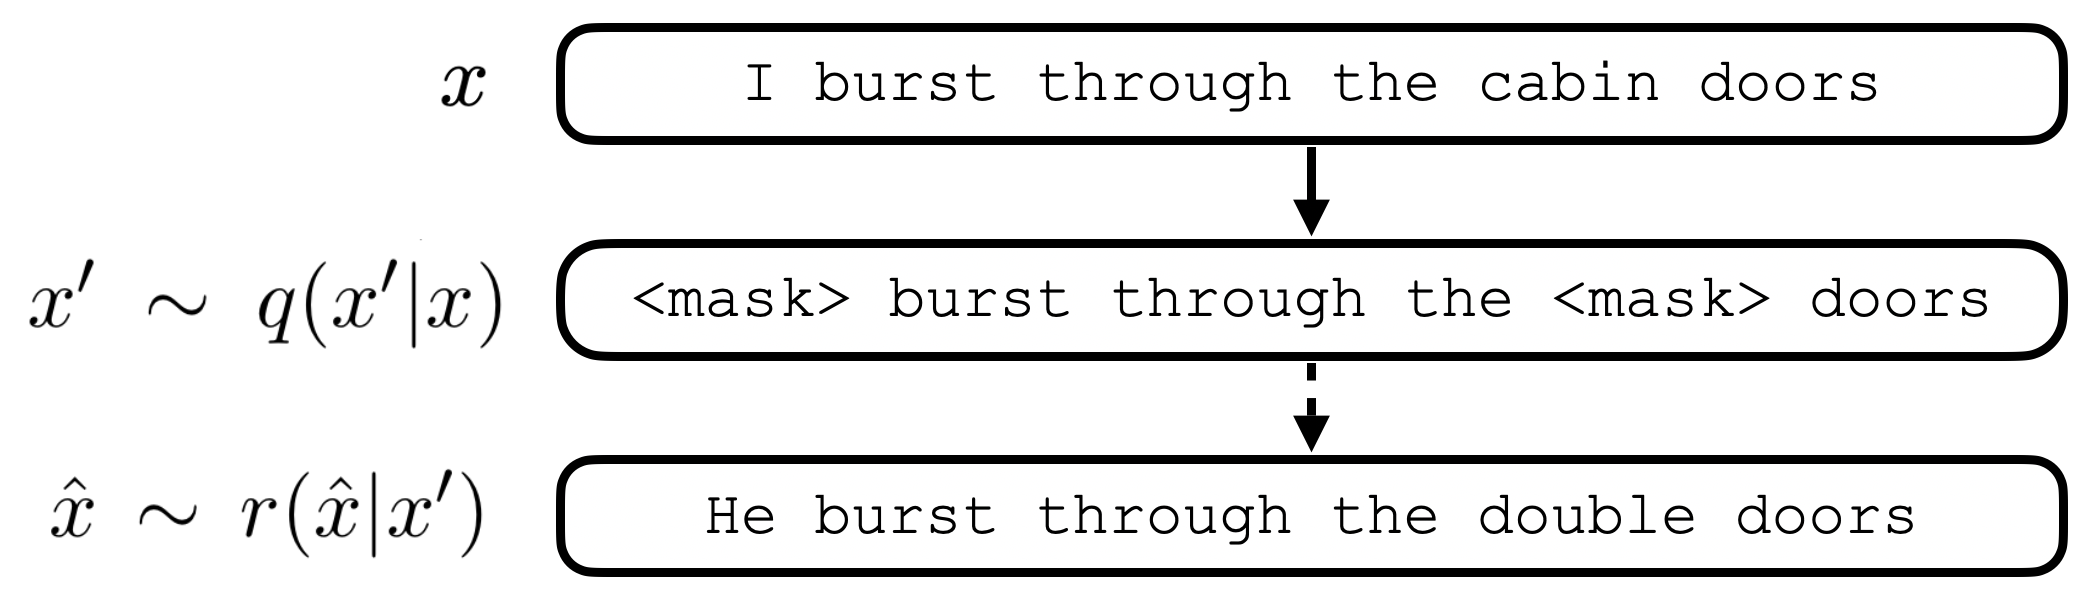
\includegraphics[scale=0.21]{img/bert_dae.png}
\caption{To sample from an MLM DAE, we apply the MLM corruption $q$ to the original sentence then reconstruct the corrupted sentence using our DAE $r$.}
\label{fig:dae_sampling}
\end{figure}

\subsection{Sampling from Denoising Autoencoders}
A denoising autoencoder (DAE) is an autoencoder trained to reconstruct a clean input $x$ from a stochastically corrupted one $x'\sim q(x'|x)$ by learning a conditional distribution $P_\theta (x| x')$ \citep{vincent2008extracting}.
We can sample from a DAE by successively corrupting and reconstructing an input using the following pseudo-Gibbs Markov chain: $x_t' \sim q(x'|x_{t-1})$, $x_t \sim P_\theta(x|x'_t).$
\comment{
\begin{align*}
    x_t' &\sim q(x'|x_{t-1})\\
    x_t &\sim P_\theta(x|x'_t) 
\end{align*}
}
As the number of training examples increases, the asymptotic distribution $\pi_n(x)$ of the generated samples approximate the true data-generating distribution $P(x)$ \citep{bengio2013generalized}.
This corruption-reconstruction process allows for sampling directly along the manifold that $P(x)$ concentrates on.

\subsection{Masked Language Models}
Recent advances in unsupervised representation learning for natural language have relied on pre-training models on a \textit{masked language modeling} (MLM) objective \citep{devlin2018, liu2019roberta}.
In the MLM objective, a percentage of the input tokens are randomly corrupted and the model is asked to reconstruct the original token given its left and right context in the corrupted sentence.
We use MLMs as DAEs \citep{lewis2019bart} to sample from the underlying natural language distribution by corrupting and reconstructing inputs (Figure \ref{fig:dae_sampling}).


\section{Combinatorial Constructions}
\label{sec:combinatorial}


%                I feel like we need some chart here to show how precision scales intuitively for folks (i.e, what’s in the experiments could come up here).

%                Hyperbolics produce low distortion and even low MAP for short bushy… also back this up with numbers from your experiments!
%                Say that the scale is critically important here. Explain that you can simply add in a learnable scale parameter. Mention a micro experiment where it has an impact, and then comment if you think it’s important more broadly.
%            Now you can devote as much as you want to the proof. 
%                You could just give the intuition of each (the precision and the lower bound).
%                I think it’s fine to say this is the key element of the proof.  
%        Embedding trees. Figure 4 is very good. 
%            You should push credit to Abraham earlier (when you mention Steiner nodes). Our contribution is applying them to these embeddings, we build on their iddeas.
%             Line 284. Probably make the is an example environment. Make sure it’s clear the reader needs to transition.
%            Make sure this section is a little more sandwich method (you don’t tell them up front—need more signposting)

We first focus on hyperbolic tree embeddings---a natural approach
considering the tree-like behavior of hyperbolic space.  We
review the embedding of \citet{sarkar} to higher dimensions. We then
provide novel analysis about the precision of the embeddings that
reveals fundamental limits of hyperbolic embeddings. In particular, we
characterize the bits of precision needed for hyperbolic
representations. We then extend the construction to $r$ dimensions,
and we propose to use Steiner nodes to better embed general graphs as
trees building on a condition from \citet{Abraham}.

\paragraph*{Embedding trees} The nature of hyperbolic space lends itself towards excellent tree embeddings. In fact, it is possible to embed trees into the Poincar\'{e} disk $\mathbb{H}_2$ with arbitrarily low distortion \cite{sarkar}. Remarkably, trees cannot be embedded into Euclidean space with arbitrarily low distortion for \emph{any} number of dimensions. These notions motivate the following two-step process for embedding hierarchies into hyperbolic space.
\begin{enumerate}
  \setlength\itemsep{0em}
\item Embed the graph $G=(V,E)$ into a tree $T$,
\item Embed $T$ into the Poincar\'{e} ball $\mathbb{H}_d$.
\end{enumerate}

We refer to this process as the \emph{combinatorial construction}. Note that we are not required to minimize a loss function. We begin by describing the second stage, where we extend an elegant construction from \citet{sarkar}. 

\subsection{Sarkar's Construction}
Algorithm~\ref{alg:sarkar} implements a simple embedding of trees into $\mathbb{H}_2$. The algorithm takes as input a scaling factor $\tau$ a node $a$ (of degree $\operatorname{deg}(a)$) from the tree with parent node $b$. Suppose $a$ and $b$ have already been embedded into $\mathbb{H}_2$ and have corresponding embedded vectors $f(a)$ and $f(b)$. The algorithm places the children $c_1, c_2, \ldots, c_{\operatorname{deg}(a)-1}$ into $\mathbb{H}_2$ through a two-step process. 

First, $f(a)$ and $f(b)$ are reflected across a geodesic (using circle inversion) so
that $f(a)$ is mapped onto the origin $0$ and $f(b)$ is mapped onto some point $z$.
% We compute the angle of $Z'$.
Next, we place the children nodes to vectors $y_1, \ldots, y_{d-1}$ equally spaced around a circle with radius $\frac{e^\tau-1}{e^\tau+1}$ (which is a circle of radius $\tau$ in the hyperbolic metric), and maximally separated from the reflected parent node embedding $z$. Lastly, we reflect all of the points back across the geodesic. 
Note that the isometric properties of reflections imply that all children are now at hyperbolic distance exactly $\tau$ from $f(a)$.

\begin{algorithm}[t]
\begin{algorithmic}[1]
\STATE \textbf{Input:} Node $a$ with parent $b$, children to place $c_1, c_2, \ldots, c_{\operatorname{deg}(a)-1}$, partial embedding $f$ containing an embedding for $a$ and $b$, scaling factor $\tau$
\STATE $(0, z) \leftarrow \operatorname{reflect}_{f(a) \rightarrow 0}(f(a),f(b))$ %\COMMENT{circle inversion}
\STATE $\theta \leftarrow \operatorname{arg}(z)$ \hspace{2em} \COMMENT{angle of $z$ from x-axis in the plane}
\FOR{$i \in \{1, \ldots, \operatorname{deg}(a)-1 \}$}
\STATE $y_i \leftarrow \left(\frac{e^\tau-1}{e^\tau+1} \cdot \cos\left(\theta + \frac{2\pi i}{\operatorname{deg}(a)} \right) , \frac{e^\tau-1}{e^\tau+1} \cdot \sin\left(\theta+\frac{2\pi i}{\operatorname{deg}(a)}\right) \right)$ % \label{alg:sarkar:step:circle}
\ENDFOR
\STATE $(f(a), f(b), f(c_1),\ldots,f(c_{\operatorname{deg}(a)-1})) \leftarrow \operatorname{reflect}_{0 \rightarrow f(a)}(0, z, y_1, \ldots, y_{\operatorname{deg}(x)-1})$
\STATE \textbf{Output:} Embedded $\mathbb{H}_2$ vectors $f(c_1), f(c_2), \ldots, f(c_{\operatorname{deg}(a)-1})$
\end{algorithmic}
\caption{Sarkar's Construction}
\label{alg:sarkar}
\end{algorithm}

To embed the entire tree, we place the root at the origin $O$ and its children in a circle around it (as in Step~5 of Algorithm~\ref{alg:sarkar}), then recursively place their children until all nodes have been placed. Notice this construction runs in linear time.

\subsection{Analyzing Sarkar's Construction}
\label{sec:sarkar}
The \emph{Voronoi cell} around a node $a \in T$ consists of points $x \in \mathbb{H}_2$ such that $d_H(f(a),x) \leq d_H(f(b),x)$ for all $b \in T$ distinct from $a$. That is, the cell around $a$ includes all points closer to $f(a)$ than to any other embedded node of the tree. Sarkar's construction produces Delauney embeddings: embeddings where the Voronoi cells for points $a$ and $b$ touch only if $a$ and $b$ are neighbors in $T$. Thus this embedding will preserve neighborhoods.

A key technical idea exploited by \citet{sarkar} is to scale all the
edges by a factor $\tau$ before embedding. We can then recover the original distances
by dividing by $\tau$. This transformation exploits the fact that
hyperbolic space is not {\em scale invariant}.
Sarkar's construction always captures neighbors perfectly, but Figure~\ref{fig:geod} implies that increasing the scale preserves the distances between farther nodes better.
Indeed, if one sets
$\tau
= \frac{1+\varepsilon}{\varepsilon}\left(2\log \frac{\operatorname{deg}_{\max}}{\pi
/2}\right)$, then the worst-case distortion $D$ of the resulting embedding is no more than
$1+\varepsilon$. For trees, Sarkar's construction has arbitrarily high
fidelity. However, this comes at a cost: the scaling $\tau$ affects
the bits of precision required. In fact, we will show that the
precision scales logarithmically with the degree of the tree---but linearly with the maximum path length. We use
this to better understand the situations in which hyperbolic
embeddings obtain high quality.

%Algorithm~\ref{alg:sarkar} produces edges scaled by $\nu$. That is, a unit distance has been scaled to $\nu$, and we can recover the original distances by dividing by $\nu$. Choosing $\nu$ correctly allows us to bound the distortion $d_{wc}$ of the embedding to $1+\varepsilon$ for any $\varepsilon > 0$.


%We call this Sarkar's condition.

%We build on the $\mathbb{H}_2$ construction from \citet{sarkar}. This approach produces Delauney embeddings, i.e., embeddings $f$ where the Voronoi cells for points $f(x),f(y)$ \footnote{The \emph{Voronoi cell} around $f(x)$ consists of points $\alpha \in \mathbb{H}_2$ such that $d_H(f(x),\alpha) \leq d_H(f(y),\alpha)$ for all $y \in T$ distinct from $x$. That is, the cell around $f(x)$ includes all points closer to $f(x)$ than any other embedded vertex of the tree.} touch only if $x,y$ are neighbors in $T$. The basic idea is to embed the children of $x$ so that each child is placed inside a disjoint cone emanating from $x$. Moreover, the cones rooted at child $y$ lie inside the cone rooted at $x$ containing $y$, so that Voronoi cells around nodes in different subtrees cannot touch. Full details on this approach are found in \citet{sarkar}.

How many bits of precision do we need to represent points in
$\mathbb{H}_2$? If $x \in \mathbb{H}_2$, then $\|x \| < 1$, so we need
sufficiently many bits so that $1 - \|x\|$ will not be rounded to zero. This requires
roughly $-\log (1-\|x\|) = \log \frac{1}{1-\|x\|}$ bits.  Say we are
embedding two points $x,y$ at distance $d$. As described in the
background, there is an isometric reflection that takes a pair of points $(x,y)$
in $\mathbb{H}_2$ to $(0,z)$ while preserving their distance, so
without loss of generality we have that
\[ d = d_H(x, y) = d_H(0,z) = \acosh \left(1+2\frac{\|z\|^2}{1-\|z\|^2} \right). \]
Rearranging the terms, we have \[\frac{\cosh(d)+1}{2} = \frac{1}{1-\|z\|^2} \ge \frac{1/2}{1-\|z\|}.\] Thus, the number of bits we want so that $1 - \|z\|$ will not be rounded to zero is $\log ( \cosh(d)+1)$. Since $\cosh(d) = (\exp(d)+\exp(-d))/2$, this is roughly $d$ bits.
That is, in hyperbolic space, we need about $d$ bits to express distances of $d$ (rather than $\log d$ as we would in Euclidean space).%
\footnote{Although it is particularly easy to bound precision in the Poincar{\'e} model, this fact holds generally for hyperbolic space independent of model. See Appendix~\ref{app:CombinatorialProofs} for a general lower bound argument.}
This result will be of use below.

Now we consider the largest distance in the embeddings produced by Algorithm~\ref{alg:sarkar}. If the longest path in the tree is $\ell$, and each edge has length $\tau = \frac{1}{\varepsilon}\left(2\log \frac{\operatorname{deg}_{\text{max}}}{\pi /2}\right)$, the largest distance is $O(\frac{\ell}{\varepsilon}\log \operatorname{deg}_{\text{max}})$, and we require this number of bits for the representation.

We interpret this expression. Note that $\operatorname{deg}_{\max}$ is inside the $\log$ term, so that a bushy tree is not penalized much in precision. On the other hand, the longest path length $\ell$ is not, so that hyperbolic embeddings struggle with long paths. 
Moreover, by selecting an explicit graph, we derive a matching lower
bound, concluding that to achieve a distortion $\varepsilon$, any
construction requires $\Omega\left(\frac{\ell}{\varepsilon} \log (\text{deg}_{\max}) \right)$
bits, which matches the upper bound of the combinatorial
construction. The argument follows from selecting a graph consisting
of $m(\text{deg}_{\max}+1)$ nodes in a tree with a single root and $\text{deg}_{\max}$ chains each of length $m$. The
proof of this result is described in Appendix~\ref{app:CombinatorialProofs}.

%% \begin{figure}
%% \centering
%% 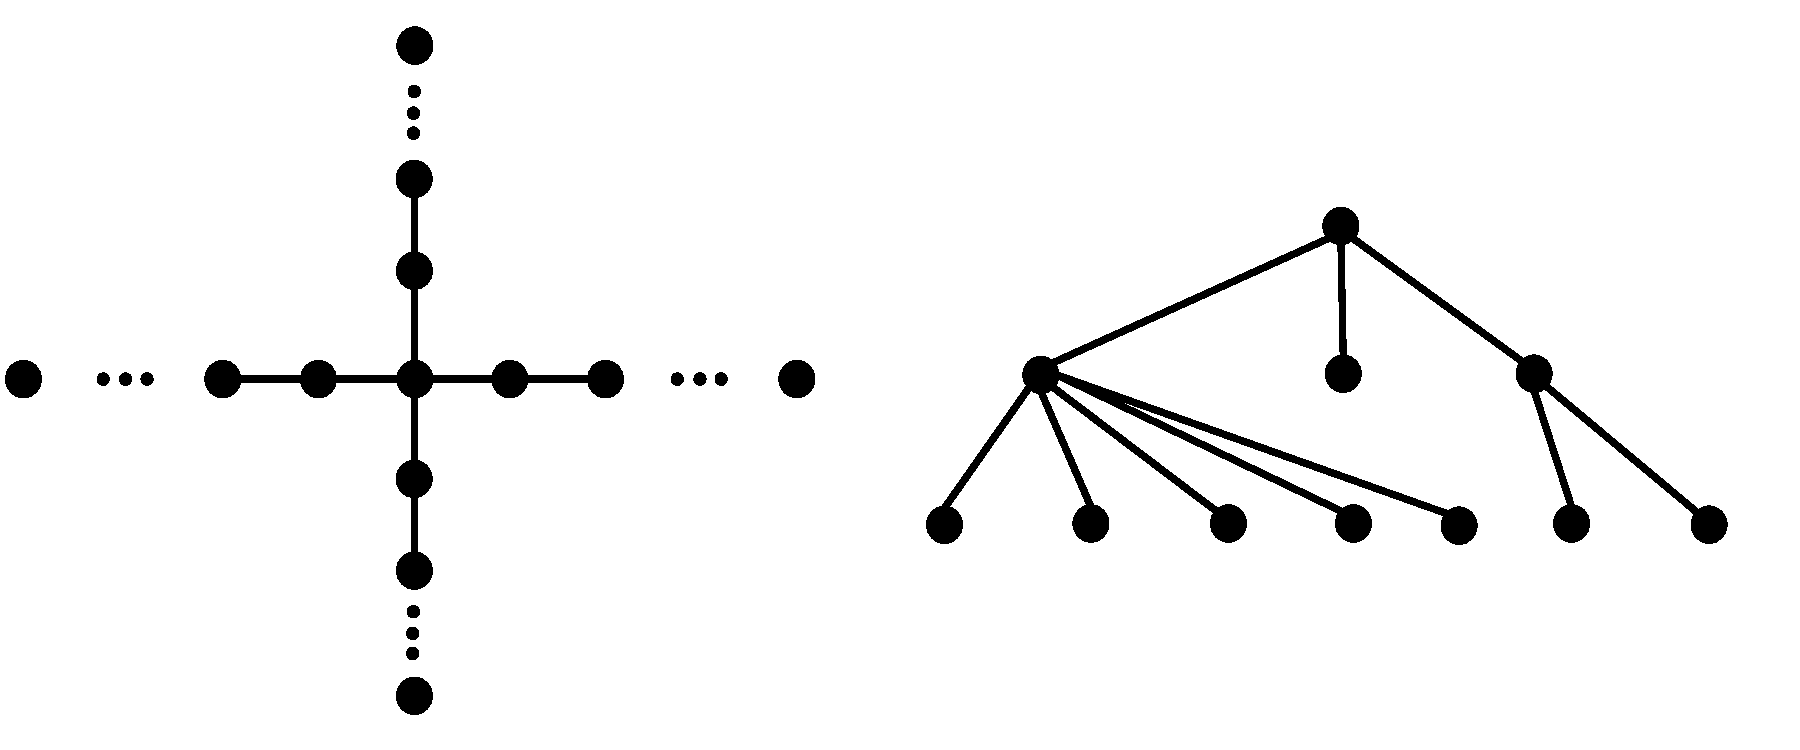
\includegraphics[width=0.50\textwidth]{figures/chain2.pdf}
%% \caption{Graphs with long chains are difficult for hyperbolic embeddings (left) while short bushy trees are easy (right).}
%% \label{fig:chains}
%% \end{figure}

%Our implementation of the construction follows \cite{Sarkar} closely, with simple modifications required by the fact that in \cite{Sarkar}, the construction is performed in (abstract) hyperbolic space, while we work with the Poincar\'{e} models. 

\subsection{Improving the Construction}



%\begin{table}[tb]
%\centering
%\begin{tabular}{|l||c|c|c|c|c|}
%\hline 
%Dataset & Nodes & $d_{\max}$ &  $r=2$ & $r=3$ & $r=5$ \\    \hline    \hline
%Bal. Tree     & 40    &4  & 25 & 13  & 13 \\ \hline
%Phy. Tree & 344  &16 & 425 & 142 & 107\\ \hline
%\end{tabular}
%\caption{Precision upper bound required for combinatorial construction at $\varepsilon=1.0$ tolerance for two trees described in Section~\ref{sec:experiments}.}
%\label{table:bitcost}
%\end{table}

Our next contribution is a generalization of the construction from the disk $\mathbb{H}_2$ to the ball $\mathbb{H}_r$. Our construction follows the same line as Algorithm~\ref{alg:sarkar}, but since we have $r$ dimensions, the step where we place children spaced out on a circle around their parent now uses a hypersphere.

Spacing out points on the hypersphere is a classic problem known as \emph{spherical coding} \cite{Spheres}. As we shall see, the number of children that we can place for a particular angle grows with the dimension. Since the required scaling factor $\tau$ gets larger as the angle decreases, we can reduce $\tau$ for a particular embedding by increasing the dimension. Note that increasing the dimension helps with bushy trees (large $\operatorname{deg}_{\max}$), but has limited effect on tall trees with small $\operatorname{deg}_{\max}$. We show

%there are $r-1$ angles $\theta_1, \ldots, \theta_{r-1}$. We divide the angles into $k$ parts, allowing us to place $\Theta(k^{r-1})$ children around any node for $k\geq 2$. Since we need $k^{r-1} \geq \operatorname{deg}_{\max}$, we can ultimately reduce the precision linearly in $r$ for $r$ up to $\leq (\log \operatorname{deg}_{\max})+1$. 


\begin{proposition} The generalized $\mathbb{H}_r$ combinatorial construction has distortion at most $1+\varepsilon$ and requires at most $O(\frac{1}{\varepsilon}\frac{\ell}{r} \log \operatorname{deg}_{\max})$ bits to represent a node component for $r \leq (\log \operatorname{deg}_{\max})+1$, and $O(\frac{1 }{\varepsilon}\ell)$ bits for $r > (\log \operatorname{deg}_{\max})+1$. 
\end{proposition}

The algorithm for the generalized $\mathbb{H}_r$ combinatorial construction replaces Step~5 in Algorithm~\ref{alg:sarkar} with a node placement step based on ideas from coding theory. The children are placed at the vertices of a hypercube inscribed into the unit hypersphere (and afterwards scaled by $\tau$). Each component of a hypercube vertex has the form $\frac{\pm 1}{\sqrt{r}}$. We index these points using binary sequences ${a} \in \{0,1\}^r$ in the following way:

\[{x}_{ a} = \left( \frac{(-1)^{a_1}}{\sqrt{r}}, \frac{(-1)^{a_2}}{\sqrt{r}} , \ldots, \frac{(-1)^{a_r}}{\sqrt{r}} \right).\]

We can space out the children by controlling the distances between the children. This is done in turn by selecting a set of binary sequences with a prescribed minimum Hamming distance---a binary error-correcting code---and placing the children at the resulting hypercube vertices. We provide more details on this technique and our choice of code in the appendix.
%\begin{proof}
%Our argument connects the required edge lengths for Sarkar's condition to be met, and the number of children we can place around a node $k^{r-1}$. We require $k^{r-1} \geq d_{\max}$.

%First, we can simplify our analysis by isometrically reflecting hyperbolic space so that the parent $x$ is the origin $0$. Let this isometry take $y$ to $p$. Then, using the hyperbolic distance formula, \begin{align*} d_H&(x,y) = d_{H}(0,q) = \\ &\mathsf{acosh}\left(1 + \frac{\cos^2 \theta/2}{1 - \cos^2 \theta/2}\right) = 
 % \mathsf{acosh}\left(1 + \cot \frac{\theta}{2}\right).\end{align*}
%Now we estimate $\exp\{ d_H(x,y) \} - 1 =  \cot \frac{\theta}{2}$ yielding $\tan \frac{\theta}{2} \leq \exp\{ - d_H(x,y) \}.$

%We place rays spaced at intervals of $\pi/k$ emanating from a point in each dimension. The cones are placed aligned with these rays. The resulting lattice can thus hold $k^{r-1}$ cones. In order to place all the children of each node, we must have $k^{r-1} \geq d_{\max}$. 
%Then, the edge lengths satisfy
%\begin{align*}
%-\log &\tan \frac{\pi}{2k} = - \log \tan \frac{\pi d_{\max}^{-1/r}}{2} \approx - \log \frac{\pi d_{\max}^{-1/r}}{2} \\
%&=  \frac{1}{r} \log d_{\max} - \log \frac{\pi}{2}.
%    \end{align*}
%We only need to meet Sarkar's condition, which offers $1+\varepsilon$ distortion if each length is scaled by the former quantity times $\frac{1+\varepsilon}{\varepsilon}$. Thus we meet our distortion bound. Next, recall that for a node component, the representation requires no more bits than the maximum path length $\ell$ times the edge length for our tree; this quantity is given by 
%\begin{equation}
%O\left(\frac{1 +  \varepsilon}{\varepsilon}\frac{\ell}{r} \log d_{\max} \right),
%\label{eq:prec}
%\end{equation}
%as desired.
%\end{proof}. 

%Observe that the precision has now been decreased by a factor of $r$, the dimension.

%To gain intuition about the precision-dimension tradeoff,
%Table~\ref{table:bitcost} shows the precision bound as the embedding dimension changes for two trees.
% The key takeaways of our analysis are:
% \begin{itemize}
%   \setlength\itemsep{0em}

% \item
% There is a fundamental tension between precision and quality in
% hyperbolic embeddings.

% \item Hyperbolic embeddings have an exponential advantage in space compared to Euclidean embeddings for short, bushy hierarchies, but will have less of an advantage
% for graphs that contain long paths.

% \item Choosing an appropriate scaling factor $\tau$ is critical for quality.
% Later, we will propose to learn this scale factor automatically for computing embeddings in PyTorch.
% \end{itemize}




\subsection{Embedding into Trees}
%Since embedding trees into the Poincar\'{e} can be performed with distortion as low as we desire, it remains to consider the distortion in the first stage. 
\begin{figure}
\centering
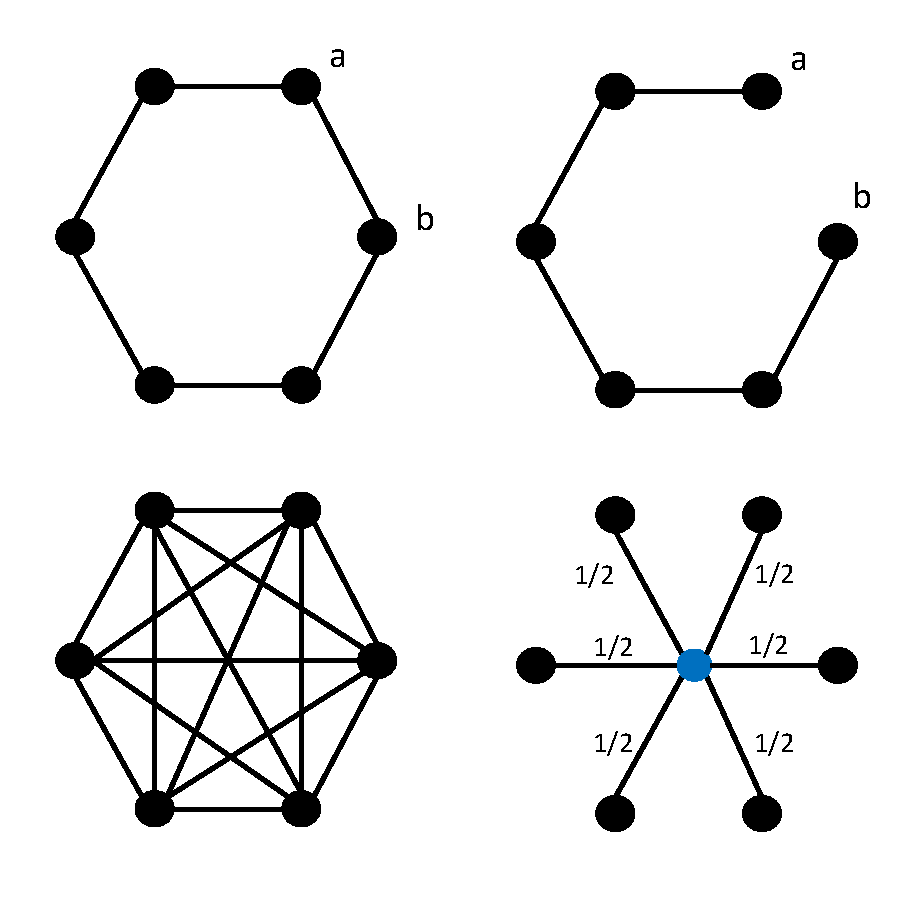
\includegraphics[width=0.3\textwidth]{figures/steiner.pdf}
\caption{Top. Cycles are a challenge for tree embeddings: $d_G(a,b)$ goes from $1$ to $5$. Bottom. Steiner nodes can help: adding a node (blue) and weighting edges maintains the pairwise distances.}
\label{fig:steiner}
\end{figure}
We revisit the first step of the construction: embedding graphs into
trees. There are fundamental limits to how well graphs can be embedded
into trees; in general, breaking long cycles inevitably adds
distortion, as shown in Figure~\ref{fig:steiner}. We are inspired by a
measure of this limit, the \emph{$\delta$-4 points condition} introduced
in \citet{Abraham}. A graph on $n$ nodes that satisfies the $\delta$-4
points condition has distortion at most $(1+\delta)^{c_1 \log n}$ for
some constant $c_1$. This result enables our end-to-end embedding to
achieve a distortion of at most \[D(f) \leq (1+\delta)^{c_1 \log n}(1
+ \varepsilon).\]

The result in \citet{Abraham} builds a tree with \emph{Steiner} nodes. These additional nodes can help control the distances in the resulting tree.
\begin{example} \label{ex:steiner}
Embed a complete graph on $\{1,2,\ldots, n\}$ into a tree. The tree will have a central node, say 1, w.l.o.g., connected to every other node; the shortest paths between pairs of nodes in $\{2,\ldots,n\}$ go from distance 1 in the graph to distance 2 in the tree. However, we can introduce a Steiner node $n+1$ and connect it to all of the nodes, with edge weights of $\frac{1}{2}$. This is shown in Figure~\ref{fig:steiner}. The distance between any pair of nodes in $\{1,\ldots,n\}$ remains 1.\end{example}

Note that introducing Steiner nodes can produce a weighted tree, but Algorithm~\ref{alg:sarkar} readily extends to the case of weighted trees by modifying Step~5.
We propose using the Steiner tree algorithm in \citet{Abraham} (used to achieve the distortion bound) for real embeddings, and we rely on it for our experiments in Section~\ref{sec:experiments}. In summary, 
the key takeaways of our analysis in this section are:
\begin{itemize}
%\setlength\itemsep{0em}
\item
There is a fundamental tension between precision and quality in
hyperbolic embeddings.

\item Hyperbolic embeddings have an exponential advantage in space compared to Euclidean embeddings for short, bushy hierarchies, but will have less of an advantage
for graphs that contain long paths.

\item Choosing an appropriate scaling factor $\tau$ is critical for quality.
Later, we will propose to learn this scale factor automatically for computing embeddings in PyTorch.
\item Steiner nodes can help improve embeddings of graphs.
\end{itemize}
%We discuss the limiting factors, mitigating these with Steiner nodes, and suitable algorithms with distortion guarantees.


%What prevents us from embedding a general graph into a tree with low distortion? The answer is long cycles. Such cycles must be broken, and the distances between the nodes adjacent to the broken edge ($a$ and $b$ in Figure~\ref{fig:steiner}) are inevitably large. Tree embeddings are therefore limited by the structure of the graph. 

%However, we can tackle this challenge by introducing \emph{Steiner} nodes, as in \citet{Abraham}. These additional nodes can help control the distances in the resulting tree:
%\begin{example} \label{ex:steiner}
%We embed a complete graph on $\{1,2,\ldots, n\}$ into a tree. The resulting tree will have a central node, say 1 w.l.o.g., connected to every other node; the shortest paths between pairs of nodes in $\{2,\ldots,n\}$ go from distance 1 in the graph to distance 2 in the tree. However, we can instead introduce a Steiner node $(n+1)$ and connect it to all of the nodes, setting edge weights of $\frac{1}{2}$. This is shown in Figure~\ref{fig:steiner}. The distance between any pair of nodes in $\{1,\ldots,n\}$ remains 1.\end{example}

%This simple example reveals the power of Steiner nodes for tree embeddings. In fact, there exist fundamental quantities measuring the best-possible tree embedding, and the algorithms that achieve these best embeddings rely on Steiner nodes. For example, the $\delta$-4 points condition is such a measure \cite{Abraham}. A graph on $n$ nodes that satisfies the $\delta$-4 points condition has distortion at most $(1+\delta)^{c_1 \log n}$ for some constant $c_1$. Since worst-case distortion is multiplicative, this enables our end-end embedding to achieve a distortion of at most  \[D \leq (1+\delta)^{c_1 \log n}(1 + \varepsilon).\]

%In other words, we have an upper bound on our overall distortion as a function of an intrinsic graph property ($\delta$) and a parameter we control ($\varepsilon$). We propose using the Steiner tree algorithm in \cite{Abraham} (used to achieve the distortion bound) for real embeddings, and we relied on it for our experiments in Section~\ref{sec:experiments}. In summary, 
%\begin{itemize}
%\item Even in general settings, consider introducing additional nodes to improve embedding quality.
%\end{itemize}
%More generally, additional nodes can improve the quality of the embedding.

%\begin{tcolorbox}
%{\bf Takeaway}: Even in general settings, we may wish to introduce extra nodes to improve embedding quality.
%\end{tcolorbox}


%There are a number of available bounds describing the distortion incurred by embedding arbitrary $n$-point metric spaces into trees \cite{Fakcharoenphol,Elkin}. However, we are particularly interested in embedding hierarchies; such graphs should offer structure that is close to tree-like. We seek a measure of tree-ness that is intrinsic to metric space and characterizes the distortion.

%There are a number of options. We rely on the $\varepsilon$-4-points condition introduced in \cite{Abraham}, where trees always achieve $\varepsilon=0$. The results in \cite{Abraham} show that a metric space $V$ on $n$ points that satisfies the $\varepsilon$-4PC for some $\varepsilon \in [0,1]$ can be embedded into a tree metric with distortion at most $(1+\varepsilon)^{c_1 \log n}$ for some constant $c_1$. Since worst-case distortion is multiplicative, the overall distortion is bounded as \[D \leq (1+\varepsilon)^{c_1 \log n}(1 + \varepsilon').\] Here we observe that $n$ and $\varepsilon$ are features of the graph, while $\varepsilon'$, the parameter controlling the hyperbolic embedding fidelity is under our control, at the cost of increasing the number of bits of precision.

%The work in \cite{Abraham} includes an algorithm that builds a Steiner tree matching the bound of $(1+\varepsilon)^{c_1 \log n}$. We implement this algorithm for the experiments detailed in Section~\ref{sec:experiments}. However, the algorithm requires $O(n^3)$ time to build a tree for $n$ points. Thus, we often opt for a simpler approach. As we shall see in our experiments, we have observed that even a simple BFS tree can be used as the embedding of choice, offering good results at a very cheap computational cost. 

%Consider four points $w,x,y,z$ in metric space $V$ ordered so that the three distance matchings $d(w,x)+d(y,z)$, $d(w,y)+d(x,z)$, $d(w,z)+d(x,y)$ satisfy $d(w,x) + d(y,z) \leq d(w,y) + d(x,z) \leq d(w,z) + d(x,y)$. Then, $V$ satisfies the $\varepsilon$-4-points condition if
%\[d(w,z) + d(x,y) \leq d(w,y) + d(x,z) + 2\varepsilon \min\{d(w,x),d(y,z)\}.\]
%That is, $\varepsilon$ measures the difference in the largest matchings, normalized by the smallest distance. Note that $\varepsilon=1$ is satisfied in all spaces $V$ by the triangle inequality. At the other extreme, if $\varepsilon=0$, the two largest distance matchings are equal and the $\varepsilon$-4PC reduces to the classical 4-points-condition \cite{Buneman}, which every tree satisfies. In other words, the $\varepsilon$ parameter reflects how tree-like the metric space $V$ is. Moreover, as shown in \cite{Abraham}, a metric space $V$ on $n$ points that satisfies the $\varepsilon$-4PC for some $\varepsilon \in [0,1]$ can be embedded into a tree metric with distortion at most $(1+\varepsilon)^{c_1 \log n}$ for some constant $c_1$.










%%%%%%%%%%%%%

%Since worst-case distortion is multiplicative, the overall distortion is bounded as \[D \leq (1+\varepsilon)^{c_1 \log n}(1 + \delta).\] Here we observe that $n$ and $\varepsilon$ are features of the graph, while $\delta$ is a parameter that we may decrease, at the cost of increasing the number of bits of precision.
% move this to appendix:
%
%\begin{proof}
%We start with the $n=1$ case. Consider any two leaf nodes
%$x,y$. First, we show that all of the leaves have equal norm, or otherwise we could equalize this distance without increasing the distortion. To see this, let the longest edge have length $b$ and the shortest have length $a$. The longest path has length at most $2a$, while the shortest path has length at least $b$. The worst-case distortion is the largest expansion (at most $2a/2 = a/1$) multiplied by the largest contraction (at worst $2/(2b)=1/b$, or $a/b$. Thus, equalizing $a/b$ can only decrease the distortion.
%
%Let $u=\|x\|$ and $\bar u = \frac{u^2}{1-u^2}$. Then, $d_{h}(0,x) =
%\mathsf{acosh}\left(1 + 2 \bar u\right)$. We then want to show that
%$\bar u = \Omega\left(\varepsilon^{-1}\right)$.
%
%We argue by considering the distance between $x$ and $y$:
%\begin{align*}
%  d_{H}(x,y) = & \mathsf{acosh}\left( 1 + 2\frac{\|x - y\|^2}{(1-\|x\|^2)(1-\|y\|^2)} \right) \\
%  = &
%  \mathsf{acosh}\left( 1 + 4(1 - \hat{x}^T\hat{y})\frac{u^2}{(1-u^2)^2} \right)
%\end{align*}
%in which $\hat{x}u = x$ and $\hat{y}u = y$.
%
%Now, since $d_{H}(x,y) \leq d_{H}(0,x) + d_{h}(0,y) = 2d_{H}(0,x)$ to achieve distortion $\varepsilon$ we must show
%\[ d_{H}(x,y) \geq 2d_{H}(0,x)(1-\varepsilon). \]
%
%We show that $\bar u =
%\Omega(\varepsilon^{-1})$, which implies we need
%$\log(\varepsilon^{-1})$ bits to represent this value, completing the $n=1$ case.
%
%Note that $\cosh$ is monotonic, so that w can write
%\begin{align*} 
%4(1 - \hat{x}^T&\hat{y})\frac{u^2}{(1-u^2)^2}\\
%& \geq \cosh(2d_{H}(0,x)(1-\varepsilon)) - 1 \\
%& =2 \left(\cosh^2(d_{H}(0,x)(1-\varepsilon)) -  1\right)
%\end{align*}
%
%
%Here, we use the estimate that
%\[ \cosh^2(z(1-\varepsilon)) \geq (1 - 2\varepsilon \cosh(z)) \cosh^{2}(z)  \]
%Next, we can write, supposing that $\hat{x}^T\hat{y} \geq 0$
%with $z=\mathrm{acosh}(1 + 2\bar u)$,
%\[ 1 + 2\frac{\bar u^2}{u^2} \geq  (1 - 2 \varepsilon (1 + 2 \bar u) )\left(1 + 2 \bar u\right)^2  \]
%\[ 0 = 2\bar u^2 {\bar u}^{-1} - 2 \bar u \geq 2 \bar u^2  + 2 \bar u- 2 \varepsilon  \left(1 + 2 \bar u\right)^3\]
%
%Now, $\frac{1}{u^2} - 1 = \frac{1 - u^2}{u^2} = \bar u^{-1}$. In turn, $\varepsilon  \geq \frac{\bar u^2 + \bar u}{(1 + 2\bar u)^3}$, that is, $\varepsilon^{-1} \leq 8 \bar u + o(\bar u)$, and we are done.
%
%Next, we consider $n>1$. Observe that $d_{H}(nx,ny) = \Omega\left( \varepsilon^{-1} n\right)$ by a similar argument. {\color{red} more details}.
%\[ d(0,x) = n\varepsilon^{-1} \implies 1 + 2 \frac{\|x\|^2}{1 - \|x\|^2} \geq \exp( n \varepsilon^{-1} ) \]
%
%Thus, we need $\Omega(n \varepsilon^{-1})$ bits to represent these
%numbers. %Note, that in general to support a dynamic range of {\em hyperbolic distances $d$}, we need $\Omega(d)$ bits.
%\end{proof}





\section{Hyperbolic Multidimensional Scaling}
\label{sec:MDS}
In this section, we explore a fundamental and more general question than we did in the previous section: if we are given the pairwise distances arising from a set of points in hyperbolic space, can we recover the points? The equivalent problem for Euclidean distances is solved with multidimensional scaling (MDS). The goal of this section is to analyze the \emph{hyperbolic MDS} (h-MDS) problem. We describe and overcome the additional technical challenges imposed by hyperbolic distances, and show that exact recovery is possible and interpretable.
Afterwards we propose a technique for dimensionality reduction using principal geodesics analysis (PGA) that provides optimization guarantees.
In particular, this addresses the shortcomings of h-MDS when recovering points that do not exactly lie on a hyperbolic manifold.
%proceed to analyze perturbations for h-MDS (i.e., recovery from noisy distances), mirroring the analysis of MDS robustness.

\subsection{Exact Hyperbolic MDS}
\label{sec:exactmds}


Suppose that there is a set of
hyperbolic points $x_1,\dots, x_n \in \mathbb{H}_r$, embedded in the Poincar{\'e} ball and written $X \in
\mathbb{R}^{n \times r}$ in matrix form.
We observe all the pairwise distances $d_{i,j} = d_H(x_i, x_j)$, but do not observe $X$:
our goal is use the observed $d_{i,j}$'s to recover $X$ (or some other set of points with the same pairwise distances $d_{i,j}$).

The MDS algorithm in the Euclidean setting makes an important
\emph{centering}%
\footnote{We say that points are centered at a particular mean
  if this mean is at $0$. The act of centering refers to applying an isometry
  that makes the mean of the points $0$.}
assumption.
That is it assumes the points have mean $0$, and it turns out that if an exact
embedding for the distances exists, it can be recovered from a matrix factorization.
In other words, Euclidean MDS always recovers a centered embedding.

In hyperbolic space, the same algorithm does not work, but we show that it is possible to find an embedding centered at a different mean. 
More precisely, we introduce a new mean which we call the \emph{pseudo-Euclidean mean}, that behaves like the Euclidean mean in that it enables recovery through matrix factorization.
Once the points are recovered in hyperbolic space, they can be recentered around a more canonical mean by translating it to the origin.

Algorithm~\ref{alg:new_hmds} is our complete algorithm, and for the remainder of
this section we will describe how and why it works.
We first describe the \emph{hyperboloid model}, an alternate but equivalent model of hyperbolic geometry in which h-MDS is simpler. Of course, we can easily convert between the hyperboloid model and the Poincar\'{e} ball model we have used thus far.
Next, we show how to reduce the problem to a standard PCA problem, which recovers an embedding centered at the points' pseudo-Euclidean mean.
Finally, we discuss the meaning and implications of centering and prove that the algorithm preserves submanifolds as well---that is, if there is an exact embedding in $k < r$ dimensions centered at their canonical mean,
then our algorithm will recover them.

\paragraph*{The hyperboloid model}
Define $Q$ to be the diagonal matrix in $\R^{r+1}$ where $Q_{00} = 1$ and $Q_{ii} = -1$ for $i > 0$.
For a vector $x \in \R^{r+1}$, $x^TQx$ is called the \emph{Minkowski quadratic form}.
The hyperboloid model is defined as
\[
  \mathbb{M}_r = \left\{ x \in \R^{r+1} \middle| x^T Q x = 1 \land x_0 > 0 \right\}.
\]
This manifold is endowed with a distance measure
\[
  d_H(x, y) = \acosh(x^T Q y).
\]
As a notational convenience, for a point $x \in \mathbb{M}_r$ we will let $x_0$ denote $0$th coordinate $e_0^T x$, and let $\vec x \in \R^r$ denote the rest of the coordinates.
Notice that $x_0$ is just a function of $\vec x$ (in fact, $x_0 = \sqrt{1 + \| \vec{x} \|^2}$), and so we can equivalently consider just $\vec x$ as being a member of a model of hyperbolic space: this model is sometimes known as the Gans model.
With this notation, the Minkowski quadratic form can be simplified to $x^T Q y = x_0 y_0 - \vec{x}^T \vec{y}$.

\paragraph*{A new mean}
We introduce the new mean that we will use.
Given points $x_1, x_2, \ldots, x_n \in \mathbb{M}_r$ in hyperbolic space,
define a variance term
\[
  \Psi(z; x_1, x_2, \ldots, x_n)
  =
  \sum_{i=1}^n \sinh^2(d_H(x_i, z)).
\]
Using this, we define a \emph{pseudo-Euclidean mean} to be any local minimum of this expression.
% This is a type of \emph{Karcher mean} in hyperbolic space.%
% \footnote{A Karcher mean is a local minimum of...}
% \[
%   A(x_1, \ldots, x_n)
%   =
%   \arg \min_{z \in \mathbb{M}_r} \Psi(z; x_1, \ldots, x_n).
% \]
Notice that this average is independent of the model of hyperbolic space that we are using, since it only is defined in terms of the hyperbolic distance function $d_H$.

\begin{lemma}
  \label{lmm:pe-centered}
  Define the matrix $X \in \R^{n \times r}$ such that $X^T e_i = \vec{x}_i$ and the vector $u \in \R^n$ such that $u_i = x_{0,i}$.
  Then
  \begin{align*}
    \left. \nabla_{\vec{z}} \Psi(z; x_1, x_2, \ldots, x_n) \right|_{\vec{z} = 0}
    =
    -2 \sum_{i=1}^n x_{0,i} \vec{x}_i
    =
    -2 X^T u.
  \end{align*}
\end{lemma}
This means that $0$ is a pseudo-Euclidean mean if and only if $0 = X^T u$.
Call some hyperbolic points $x_1, \ldots, x_n$ \emph{pseudo-Euclidean centered} if their average is $0$ in this sense: i.e. if $X^T u = 0$.
We can always center a set of points without affecting their pairwise distances by simply finding their average, and then sending it to $0$ through an isometry.

\paragraph*{Recovery via matrix factorization}
Suppose that there exist points $x_1, x_2, \ldots, x_n \in \mathbb{M}_r$
for which we observe their pairwise distances $d_H(x_i, x_j)$.
From these, we can compute the matrix $Y$ such that
\begin{equation}
  \label{eq:hmds-Y}
  Y_{i,j} = \cosh\left( d_H(x_i, x_j) \right) = x_i^T Q x_j = x_{0,i} x_{0,j} - \vec{x_i}^T \vec{x_j}.
\end{equation}
Furthermore, defining $X$ and $u$ as in Lemma~\ref{lmm:pe-centered},
then we can write $Y$ in matrix form as
\begin{equation}
  \label{eq:hmds-Y2}
  Y = u u^T - X X^T.
\end{equation}
Without loss of generality, we can suppose that the points we are trying to recover, $x_1, \ldots, x_n$, are centered at their pseudo-Euclidean mean, so that $X^T u = 0$ by Lemma~\ref{lmm:pe-centered}.

This implies that $u$ is an eigenvector of $Y$ with positive eigenvalue, and the rest of $Y$'s eigenvalues are negative.
Therefore an eigendecomposition of $Y$ will find $u,\hat{X}$ such that $Y = u u^T - \hat{X} \hat{X}^T$,
i.e. it will directly recover $X$ up to rotation.

In fact, running PCA on $-Y = X^T X - u u^T$ to find the $n$ most significant non-negative eigenvectors will recover $X$ up to rotation,
and then $u$ can be found by leveraging the fact that $x_0 = \sqrt{1 + \| \vec{x} \|^2}$.

This leads to Algorithm~\ref{alg:new_hmds}, with optional post-processing steps for converting the embedding to the Poincar{\'e} ball model and for re-centering the points.
% First, this algorithm returns an embedding in the Gans model; they can be converted to the Poincar{\'e} disk model with a simple projection.
% Second, once we've recovered the points centered at their pseudo-Euclidean mean, we can recover the points centered at any other mean by reflecting it onto the origin.


\paragraph*{A word on centering}
The MDS algorithm in Euclidean geometry returns points centered at their \emph{Karcher mean} $z$, which is a point minimizing $\sum d^2(z, x_i)$ (where $d$ is the distance metric).
The Karcher center is particularly useful for interpreting dimensionality reduction; for example, we use the analogous hyperbolic Karcher mean to perform PGA in Section~\ref{sec:PGA}.

Although Algorithm~\ref{alg:new_hmds} returns points centered at their pseudo-Euclidean mean instead of their Karcher mean, they can be easily recentered
by finding their Karcher mean and reflecting it onto the origin. 
Furthermore, we show that Algorithm~\ref{alg:new_hmds} \emph{preserves the dimension of the embedding}.
More precisely, we prove Lemma~\ref{lmm:hmds-centering} in Appendix~\ref{sec:mds-proof}.
\begin{lemma}
  \label{lmm:hmds-centering}
  If a set of points lie in a dimension-$k$ geodesic submanifold, then both their Karcher mean and their pseudo-Euclidean mean lie in the same submanifold.
\end{lemma}
This implies that centering with the pseudo-Euclidean mean preserves geodesic submanifolds:
If it is possible to embed distances in a dimension-$k$ geodesic submanifold centered and rooted at a Karcher mean, then it is also possible to embed the distances in a dimension-$k$ submanifold centered and rooted at a pseudo-Euclidean mean, and vice versa.


\begin{algorithm}[t]
% \caption{h-MDS}
\caption{ }
\begin{algorithmic}[1]
\STATE {\bfseries Input: Distance matrix $d_{i,j}$ and rank $r$}
\STATE Compute scaled distance matrix $Y_{i,j} = \cosh(d_{i,j})$
\STATE $X \rightarrow \text{PCA}(-Y,r)$
\STATE Project $X$ from hyperboloid model to Poincar\'{e} model: $x \to \frac{x}{1 + \sqrt{1 + \|x\|^2}}$
\STATE If desired, center $X$ at a different mean (e.g. the Karcher mean)
\STATE \textbf{return} $X$
\end{algorithmic}
\label{alg:new_hmds}
\end{algorithm}


%%% Local Variables:
%%% mode: latex
%%% TeX-master: "hyperbolic_arxiv"
%%% End:

\subsection{Reducing Dimensionality with PGA}
\label{sec:PGA}
%{\color{red} This will get longer, with a result}.
Sometimes we are given a
high-rank embedding (resulting from h-MDS, for example), and wish to
find a lower-rank version.
In Euclidean space, one can get the optimal
lower rank embedding by simply discarding components. However, this
may not be the case in hyperbolic space.
Motivated by this, we study dimensionality reduction in hyperbolic space.

As hyperbolic space does not have a linear subspace structure like
Euclidean space, we need to define what we mean by lower-dimensional.
We follow Principal Geodesic Analysis~\cite{PGA}, \cite{GPCA}. Consider an initial
embedding with points $x_1,\dots,x_n \in \mathbb{H}_2$ and let $d_{H}
: \mathbb{H}_2 \times \mathbb{H}_2 \to \mathbb{R}_{+}$ be the hyperbolic distance.
Suppose we want to map this embedding onto a one-dimensional subspace. (Note that
we are considering a two-dimensional embedding and one-dimensional subspace
here for simplicity, and these
results immediately extend to higher dimensions.) In this case, the goal of PGA
is to find a geodesic $\gamma :
[0,1] \to \mathbb{H}_2$ that passes through the mean of the points and that minimizes the squared error (or variance):
\[ f(\gamma) = \sum_{i=1}^n \min_{t \in [0,1]} d_{H}(\gamma(t),x_i)^2 .\]
This expression can be simplified significantly and reduced to a
minimization in Euclidean space.  First, we find the mean of the
points, the point $\bar x$ which minimizes $\sum_{i=1}^n d_{H}(\bar
x, x_i)^2$; this definition in terms of distances generalizes the mean in Euclidean space.\footnote{As we noted earlier, considering the distances
without squares leads to a non-continuously-differentiable
formulation.}  Next, we reflect all the points $x_i$ so that their
mean is $0$ in the Poincar{\'e} disk model; we can do this using a
circle inversion that maps $\bar x$ onto $0$.
In the Poincar{\'e} disk model, a geodesic through
the origin is a Euclidean line, and the action of the reflection across
this line is the same in both Euclidean and hyperbolic space. Coupled
with the fact that reflections are isometric, if $\gamma$ is a line
through $0$ and $R_\gamma$ is the reflection across $\gamma$, we have
\[
  d_H(\gamma, x) = \min_{t \in [0,1]} d_H(\gamma(t), x) = \frac{1}{2} d_H(R_l x, x).
\]
Combining this with the Euclidean reflection formula and the hyperbolic metric produces
\[
  f(\gamma) = \frac{1}{4} \sum_{i=1}^n \acosh^2\left( 1 + \frac{ 8 d_{E}(\gamma,x_i)^2 }{(1 - \| x_i \|^2)^2} \right),
\]
in which $d_{E}$ is the Euclidean distance from a point to a line. If
we define $w_i = \sqrt{8} x_i / (1 - \| x_i \|^2)$ this reduces to the simplified expression
\[
  f(\gamma) = \frac{1}{4} \sum_{i=1}^n \acosh^2\left( 1 + d_{E}(\gamma,w_i)^2 \right).
\]
  
Notice that \emph{the loss function is not convex}. We observe that
there can be multiple local minima that are attractive and stable, in
contrast to PCA.  Figure~\ref{fig:pga} illustrates this nonconvexity
on a simple dataset in $\mathbb{H}_2$ with only four examples.  This
makes globally optimizing the objective difficult.
\begin{figure}
\centering
\resizebox{0.48\textwidth}{!}{\large% GNUPLOT: LaTeX picture with Postscript
\begingroup
  \makeatletter
  \providecommand\color[2][]{%
    \GenericError{(gnuplot) \space\space\space\@spaces}{%
      Package color not loaded in conjunction with
      terminal option `colourtext'%
    }{See the gnuplot documentation for explanation.%
    }{Either use 'blacktext' in gnuplot or load the package
      color.sty in LaTeX.}%
    \renewcommand\color[2][]{}%
  }%
  \providecommand\includegraphics[2][]{%
    \GenericError{(gnuplot) \space\space\space\@spaces}{%
      Package graphicx or graphics not loaded%
    }{See the gnuplot documentation for explanation.%
    }{The gnuplot epslatex terminal needs graphicx.sty or graphics.sty.}%
    \renewcommand\includegraphics[2][]{}%
  }%
  \providecommand\rotatebox[2]{#2}%
  \@ifundefined{ifGPcolor}{%
    \newif\ifGPcolor
    \GPcolortrue
  }{}%
  \@ifundefined{ifGPblacktext}{%
    \newif\ifGPblacktext
    \GPblacktextfalse
  }{}%
  % define a \g@addto@macro without @ in the name:
  \let\gplgaddtomacro\g@addto@macro
  % define empty templates for all commands taking text:
  \gdef\gplbacktext{}%
  \gdef\gplfronttext{}%
  \makeatother
  \ifGPblacktext
    % no textcolor at all
    \def\colorrgb#1{}%
    \def\colorgray#1{}%
  \else
    % gray or color?
    \ifGPcolor
      \def\colorrgb#1{\color[rgb]{#1}}%
      \def\colorgray#1{\color[gray]{#1}}%
      \expandafter\def\csname LTw\endcsname{\color{white}}%
      \expandafter\def\csname LTb\endcsname{\color{black}}%
      \expandafter\def\csname LTa\endcsname{\color{black}}%
      \expandafter\def\csname LT0\endcsname{\color[rgb]{1,0,0}}%
      \expandafter\def\csname LT1\endcsname{\color[rgb]{0,1,0}}%
      \expandafter\def\csname LT2\endcsname{\color[rgb]{0,0,1}}%
      \expandafter\def\csname LT3\endcsname{\color[rgb]{1,0,1}}%
      \expandafter\def\csname LT4\endcsname{\color[rgb]{0,1,1}}%
      \expandafter\def\csname LT5\endcsname{\color[rgb]{1,1,0}}%
      \expandafter\def\csname LT6\endcsname{\color[rgb]{0,0,0}}%
      \expandafter\def\csname LT7\endcsname{\color[rgb]{1,0.3,0}}%
      \expandafter\def\csname LT8\endcsname{\color[rgb]{0.5,0.5,0.5}}%
    \else
      % gray
      \def\colorrgb#1{\color{black}}%
      \def\colorgray#1{\color[gray]{#1}}%
      \expandafter\def\csname LTw\endcsname{\color{white}}%
      \expandafter\def\csname LTb\endcsname{\color{black}}%
      \expandafter\def\csname LTa\endcsname{\color{black}}%
      \expandafter\def\csname LT0\endcsname{\color{black}}%
      \expandafter\def\csname LT1\endcsname{\color{black}}%
      \expandafter\def\csname LT2\endcsname{\color{black}}%
      \expandafter\def\csname LT3\endcsname{\color{black}}%
      \expandafter\def\csname LT4\endcsname{\color{black}}%
      \expandafter\def\csname LT5\endcsname{\color{black}}%
      \expandafter\def\csname LT6\endcsname{\color{black}}%
      \expandafter\def\csname LT7\endcsname{\color{black}}%
      \expandafter\def\csname LT8\endcsname{\color{black}}%
    \fi
  \fi
    \setlength{\unitlength}{0.0500bp}%
    \ifx\gptboxheight\undefined%
      \newlength{\gptboxheight}%
      \newlength{\gptboxwidth}%
      \newsavebox{\gptboxtext}%
    \fi%
    \setlength{\fboxrule}{0.5pt}%
    \setlength{\fboxsep}{1pt}%
\begin{picture}(7200.00,3960.00)%
    \gplgaddtomacro\gplbacktext{%
      \csname LTb\endcsname%
      \put(682,704){\makebox(0,0)[r]{\strut{}$5$}}%
      \put(682,1131){\makebox(0,0)[r]{\strut{}$6$}}%
      \put(682,1559){\makebox(0,0)[r]{\strut{}$7$}}%
      \put(682,1986){\makebox(0,0)[r]{\strut{}$8$}}%
      \put(682,2413){\makebox(0,0)[r]{\strut{}$9$}}%
      \put(682,2840){\makebox(0,0)[r]{\strut{}$10$}}%
      \put(682,3268){\makebox(0,0)[r]{\strut{}$11$}}%
      \put(682,3695){\makebox(0,0)[r]{\strut{}$12$}}%
      \put(1428,484){\makebox(0,0){\strut{}0}}%
      \put(2634,484){\makebox(0,0){\strut{}$\pi/2$}}%
      \put(3840,484){\makebox(0,0){\strut{}$\pi$}}%
      \put(5047,484){\makebox(0,0){\strut{}$3\pi/2$}}%
      \put(6253,484){\makebox(0,0){\strut{}2$\pi$}}%
      \put(3885,918){\makebox(0,0)[l]{\strut{}non-global minima}}%
    }%
    \gplgaddtomacro\gplfronttext{%
      \csname LTb\endcsname%
      \put(176,2199){\rotatebox{-270}{\makebox(0,0){\strut{}PGA loss $f(\gamma)$}}}%
      \put(3808,154){\makebox(0,0){\strut{}angle of geodesic $\gamma$}}%
      \csname LTb\endcsname%
      \put(6344,3522){\makebox(0,0)[r]{\strut{}global minima}}%
    }%
    \gplbacktext
    \put(0,0){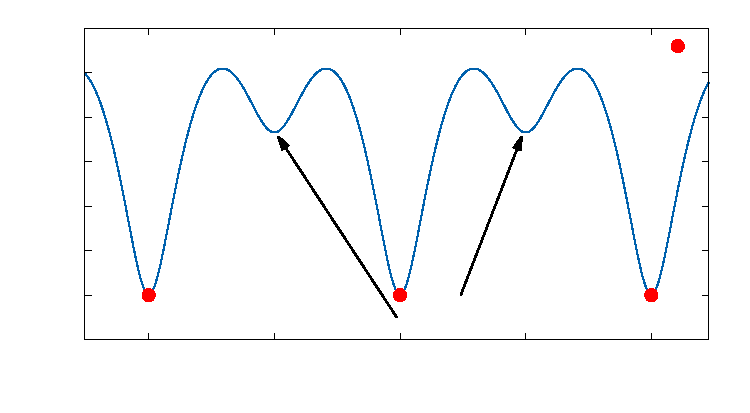
\includegraphics{gp/plotpga-eps-converted-to.pdf}}%
    \gplfronttext
  \end{picture}%
\endgroup
}
%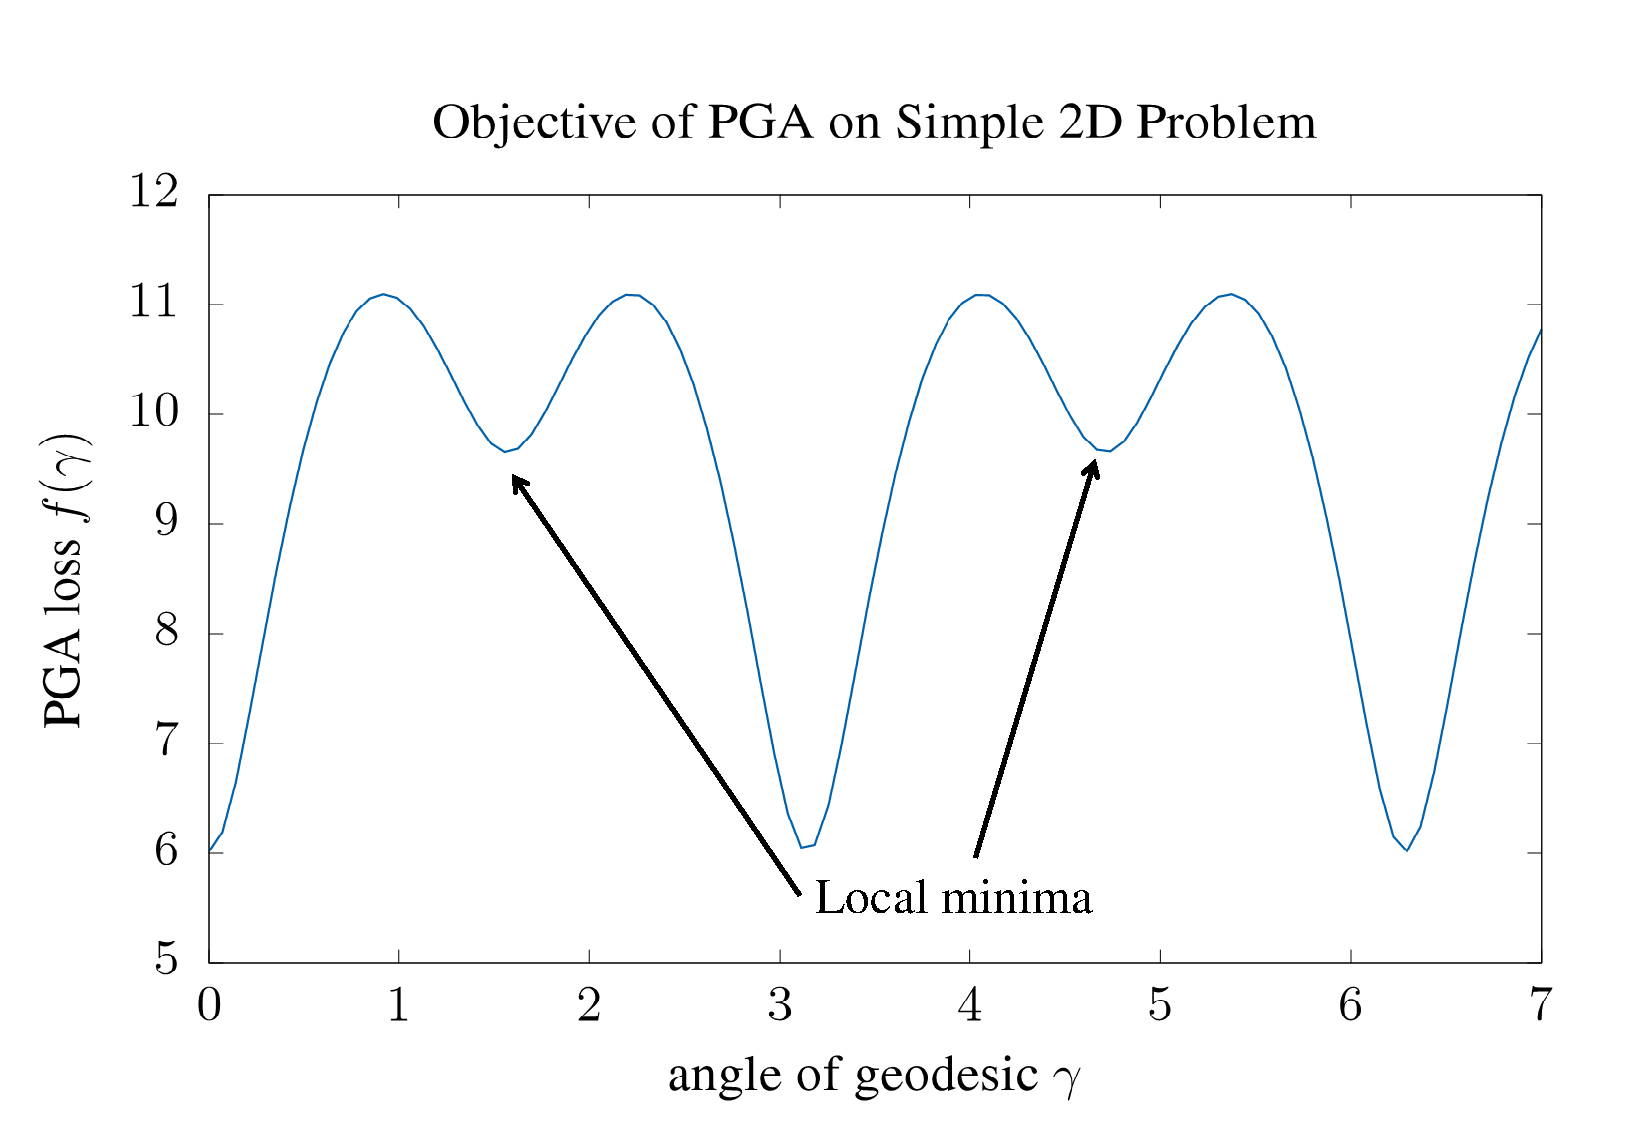
\includegraphics[width=0.3\textwidth]{gp/plotpga-labeled}
\caption{The PGA objective of an example task where the input dataset in the Poincar{\'e} disk is $x_1 = (0.8,0)$, $x_2 = (-0.8,0)$, $x_3 = (0,0.7)$ and $x_4 = (0,-0.7)$. Note the presence of non-optimal local minima, unlike PCA.}
\label{fig:pga}
\end{figure}

Nevertheless, there will always be a region $\Omega$ containing a
global optimum $\gamma^*$ that is convex and admits an efficient
projection, and where $f$ is convex when restricted to $\Omega$. Thus
it is possible to build a gradient descent-based algorithm to recover
lower-dimensional subspaces: for example, we built a simple optimizer
in PyTorch.  We also give a sufficient condition on the data for $f$ above
to be convex.
\begin{lemma}
For hyperbolic PGA if for all $i$,
\[
  \acosh^2\left( 1 + d_{E}(\gamma,w_i)^2 \right) < \min\left(1, \frac{1}{3} \| w_i \|^2 \right)
\]
then $f$ is locally convex at $\gamma$.
\label{lemma:pga}
\end{lemma}
As a result, if we initialize in and optimize over a region that
contains $\gamma^*$ and where the condition of Lemma~\ref{lemma:pga}
holds, then gradient descent will be guaranteed to converge to
$\gamma^*$. We can turn this result around and read it as a recovery
result: if the noise is bounded in this regime, then we are able to
provably recover the correct low-dimensional embedding.


% Another way of solving PGA is to approximate $f(\gamma)$ with a series of Euclidean PCA problems.
% Since the function $h(\beta) = \acosh^2(1 + \beta)$ is concave, for any $\gamma_0$
% \[
%   f(\gamma)
%   \le
%   \frac{1}{4} \sum_{i=1}^n
%   h'\left( d_{E}^2(\gamma_0,v_i)^2 \right)
%   d_{E}^2(\gamma,v_i)^2
%   +
%   R(\gamma_0, v_i)
% \]
% for some remainder $R$ that is independent of $\gamma_0$.
% This upper bound can be minimized over $\gamma$ as a weighted PCA problem, and by repeating this procedure we can converge to the optimum.

% not sure if we have space for the rest of the analysis here

%In this section, we consider how to reduce the dimensionality of embeddings. That is, we are given an embedding and wish to find a lower-rank version.
%%In Euclidean space, one can get the optimal lower rank embedding by simply discarding components. However, this may not be the case in hyperbolic space.
%%We describe a sufficient condition for dimensionality reduction to work and analyze the underlying issues. 
%
%%\begin{tcolorbox}
%%{\bf Takeaway}: Reoptimize lower dimensional embeddings.
%%\end{tcolorbox}
%
%%We work in $\mathbb{H}_2$ for simplicity, but the ideas in this section extend to higher dimensions. We are given an initial embedding 
%with points $x_1,\dots,x_n \in \mathbb{H}_2$. Our goal is to find a geodesic $\gamma : [0,1] \to \mathbb{H}_2$ that minimizes the
%variance to the points
%    \[ f(\gamma) = \sum_{i=1}^n \min_{t \in [0,1]} d_{H}(\gamma(t),x_i)^2 .\]
%    
%A major challenge that we face is that \emph{the loss function is not convex}. We observe that there
%  are multiple local minima {\color{red}PLOT}. Moreover, notice these losses are
%   attractive and stable, in contrast to analogous settings like PCA.
%
%\begin{tcolorbox}
%{\bf Takeaway}:   The underlying optimization may be nonconvex and this issue is not easily handled.
%\end{tcolorbox}
%
% {\color{red}NEEDS WRITTEN}.
%We begin by reducing the problem to one in Euclidean geometry. The key observation is that geodesics through the origin are just lines. 
%Therefore we use two steps to perform the reduction: (i) center the problem and then (ii) simplify the loss using the simpler geometry at the origin.
%The centering is done by computing the mean (known as the Frechet or Karcher
%mean)  efficiently using existing algorithms
%  
%In the Euclidean setting, we seek to find the line that minimizes the hyperbolic distances to
%  that line. The closest point to a line is half the distance of its reflection. Moreover,
%    any line is a geodesic in both Euclidean and hyperbolic geometry, hence:
%    \[ \min_{t} d_{H}(\gamma(t),x) = \frac{1}{2} \mathsf{acosh}\left(1 + \frac{d_{E}^2(l,x)}{ (1-\|x\|^2)^2 }\right) \]
%     Here, we have also used the fact that a point and its reflection have the
%     same norm. Now our expression is in terms of the Euclidean distance
%     to the line.
%
%Next, observe that we can normalize the points $v_i =
%       \frac{x_i}{1-\|x_i\|^2}$ to rewrite the above cost as $ \frac{1}{2} \mathrm{acosh}(1 + d^2_E(l,v_i) )$.
%        
%Intuitively, if there is such a line such that it's
%  variances to all points are small, then we should be able to recover
%  it. More precisely, we are looking for a set $\Omega \subseteq
%  \mathbb{S}^2$ that has three properties: (i) If there is a solution $u_*$ such that $f(u_*) = 0$, then
%      $\Omega$ contains $u_*$.(ii) The set $\Omega$ is a convex and admits an efficient projection. (iii) The loss $f$ is convex restricted to the set $\Omega$. Here,
%      \[ f(u) = \sum_{i=1}^{n} \min d_{H}( \ell(u),x_i)^2. \]
%
%We show that if there is a solution $u_*$ such that
%  \[ \sum_{i=1}^{n} r_i(u_*) \leq \min \{1, \frac{1}{3}\|v_i\|^2 \}. \]
%
%%Note that PCA does the wrong thing on the following example:
% % There are four points $y_{i} = \pm \alpha e_1$ (two of each) and two
% % of $x_i = \beta e_2$. Hence, the PCA loss for chosing $e_1$ is
% % $2\beta^2$ versus $4\alpha^2$ versus the $2\acosh(1+\beta^2)$ versus
% % $4\acosh(1+\alpha^2)^2$. Thus, we need to find values in which:
%  %\[ \beta^2 < 2 \alpha^2 \text{ and }  \acosh(1+\beta^2)^2 > 2\acosh(1+\alpha^2)^2 \]
%  %Take values like $\alpha = 5$ and $\beta = 10$.
%  
%%  We show that so long as there is a solution $u_*$ such that
%%  (\yell{see condition below}.)
%
%Thus we introduce the following straightforward algorithm.
%  \begin{itemize}
%\item Normalize the data as described in the note.
%  \item find a direction $u$:
%  \[ \min_{u \in \mathbb{S}^{n-1}} \max_{i} \|(I-uu^T)x_i\|^2 \]
%\item If the objective value is greater than $\frac{1}{3}$, fail.
%  \item If the objective value is smaller, then run projected gradient
%    descent with $P_{\Omega}$ as the projection on the original
%    function initialized with $u$.
%  \end{itemize}

%
%\subsection{Computing Derivatives}
%
%\[ r_i(u) = \| w - \|u\|^{-2}u (u \cdot w)\|^2 = \|w\|^2 - \|u\|^{-2} (u \cdot w)^2 \]
%\begin{align*}
%  h(x) = & \acosh(1+x)^2\\
%  h'(x) = & 2\acosh(1+x)(x^2 + 2x)^{-1/2}\\
%  h''(x) = & 2\left(\frac{1}{x^2 + 2x} - \acosh(1+x)(x^2 + 2x)^{-3/2}(x+1)\right)\\
%         = & 2\left(\frac{q^{1/2} - \acosh(1+x)(x+1)}{q^{3/2}}\right)\\
%  r_i(u) = & \|w_i\|^2 - (u\cdot w_i)^2 \|u\|^{-2}\\
%  r_i'(u) = & 2\|u\|^{-2} (u\cdot w_i) \left((u\cdot w_i) \|u\|^{-2} u - w_i \right) = 2\|u\|^{-2} (u\cdot w_i) (\|u\|^{-2}uu^T - I)w\\
%  r_i''(u) = & - 2w_i w_i^T \dots\\
%  f(u) = & \sum_{i=1}^{n} h(r_i(u))\\
%  f'(u) = & \sum_{i=1}^{n} h'(r_i(u))r'_i(u)\\
%  f''(u) = & \sum_{i=1}^{n} h''(r_i(u)) r'_i(u)r_i'(u)^T + h'(r_i(u))r_i''(u)\\
%  = & 2\sum_{i=1}^{n} \left(h''(r_i(u)) 2(u \cdot w_i)^2 - h'(r_i(u))\right) w_iw_i^T\\
%  = & 2\sum_{i=1}^{n} \left(h''(r_i(u)) 2(\|w_i\|^2-r_i(u)) - h'(r_i(u))\right) w_iw_i^T
%\end{align*}
%Let's do the angular version:
%\begin{align*}
%  \rho_i(\theta) = &  \|w_i\|^2(1 - \cos(\theta-\theta_i)^2) = \|w_i\|^2 \sin^2(\theta-\theta_i)\\
%  \rho_i'(\theta)= & 2 \|w_i\|^2 \sin(\theta-\theta_i) \cos(\theta-\theta_i) = \|w_i\|^2 \sin(2(\theta-\theta_i))\\
%  \rho_i''(\theta)= & 2 \|w_i\|^2 \cos(2(\theta-\theta_i))\\
%  g(\theta) = & \sum_{i=1}^{n} h(\rho_i(\theta))\\
%  g'(\theta) = & \sum_{i=1}^{n} h'(\rho_i(\theta)) \rho_i(\theta)\\
%  g''(\theta) = & \sum_{i=1}^{n} h''(\rho_i(\theta)) (\rho'_i(\theta))^2 + h'(\rho_i(\theta)) \rho''_i(\theta)\\
%  = &  \sum_{i=1}^{n} 4 \|w_i\|^4 \sin^2(2(\theta-\theta_i)) h''(\rho_i(\theta)) + 2 \|w_i\|^2 \cos(2(\theta-\theta_i)) h'(\rho_i(\theta))\\
%\end{align*}
%
%Observe that $\lim_{x \to 0} h'(x) =  2\frac{\acosh(1+x)}{\sqrt{x^2 + x}} = 2$. 
%\subsubsection{Estimates}
%
%{\bf Proposition}.  Using the notation above, 
%  \[ |\theta_i - \theta| \leq \frac{\pi}{7} \min \{ 1, \|w_i\|^{-1} \} \text{ then }
%  \frac{\partial^2}{\partial^2 \theta} h(\rho_i(\theta_i - \theta)) \geq 0
%  \] 
%
%\begin{proof}[Sketch]
%Let $\|w_i\| = t$ and, abusing notation, we write $\theta = \theta_i - \theta$ below. We show
%that when $t \leq 1$, then as long as $\theta \leq \pi/7$, then the
%term is positive definite.  We first consider when $\|w_\| = t \leq 1$
%then $h'(\rho_i(\theta)) \in [1.5,2]$ then, the second term is
%$[3t^2\cos(2\theta),4t^2\cos(2\theta)]$. We also observe that
%$h''(\rho_i(\theta)) \in [-\frac{2}{3}, -\frac{1}{3}]$. Hence, the
%lower bound for the whole term is:
%\[ \cos(2\theta) \geq \frac{8}{9} t^2 \sin^2(2\theta) \]
%Thus, this inequality holds (easily) if $\theta \in [-\pi/7,\pi/7]$.
%
%The lower bound on $h''$ still holds, hence we have:
%\[ \frac{4}{3} t^2 \sin^2(2\theta) \leq \cos(2\theta) h'(\rho(\theta)) \]
%
%For $t \geq 1$, if we insist $|\theta| \leq \pi/(7t)$ then $h'(\rho(\theta)) \geq 15/8$ and we have:
%\[ \frac{32}{45} t^2 \sin^2(2\theta) \leq \cos(2\theta) \]
%
%Note that $\sin(2\theta)^2 \leq \left(\pi/(7t)\right)^2$. It is
%straightforward to verify that the left hand side is less than $0.6$,
%while $\cos(2\pi/7) > 0.6$--and the rhs is an increasing function of $t$.
%
%\end{proof}
%
%Note that for large $t$, $\rho(t,\theta) = O(1)$ and that a constant fraction 



\section{Experiments}
\label{sec:experiments}
\section{Experiments}
\label{sec:experiments}

We validate our approach empirically, showing that our Monarch matrix parametrization achieves a favorable efficiency--accuracy tradeoff compared to baselines on a wide range of domains (text, images, PDEs, MRI), in three settings (E2E training, S2D training, and D2S fine-tuning):
\begin{itemize}[leftmargin=*,nosep,nolistsep,noitemsep]
\item
In \cref{subsec:benchmark_tasks}, on image classification and language modeling benchmarks, such as ViT / MLP Mixer on ImageNet and GPT-2 on Wikitext-103, Monarch is 2$\times$ faster to train than dense models, while achieving the same accuracy / perplexity. In \cref{subsec:pde_mri}, in scientific and medical domains where special transforms (Fourier) are common, Monarch outperforms Fourier transform based methods on PDE solving, with up to 40\% lower error, and on MRI reconstruction attains up to 15\% higher pSNR and 3.8\% higher SSIM.
\item In \cref{subsec:pde_mri}, we show that on the large OpenWebText dataset, reverse sparsification (training with Monarch weight matrices for most of the time, then transitioning to dense weight matrices) speeds up the pretraining of GPT-2 models by 2$\times$ compared to the dense model, with no loss in upstream or downstream quality.
Moreover, reverse sparsification speeds up BERT pretraining by 23\% even compared to the implementation from Nvidia that set the MLPerf~\citep{mattson2020mlperf} 1.1 record.
\item In \cref{subsec:finetuning}, as a proof of concept, we demonstrate that our Monarch approximation algorithm can improve fine-tuning efficiency for pretrained models. We show that compressing BERT to a Monarch matrix model performs comparably to a finetuned dense model on GLUE, with 2$\times$ fewer parameters and 1.7$\times$ faster finetuning speed.
\end{itemize}

\subsection{End-to-End Training}
\label{subsec:e2e_training}
\subsubsection{Benchmark Tasks: Image Classification, Language Modeling}
\label{subsec:benchmark_tasks}

We show that replacing dense matrices with Monarch matrices in ViT, MLP-Mixer, and
GPT-2 can speed up training by up to 2$\times$ without sacrificing model quality in~\cref{table:pretrain,table:gpt_pretrain}.

\textbf{Setup.} We use the popular vision benchmark, ImageNet~\citep{deng2009imagenet}. We choose recent popular Vision Transformer~\citep{dosovitskiy2020image}, and MLP-Mixer~\citep{tolstikhin2021mlp} as representative base dense models.
For language modeling, we evaluate GPT-2~\citep{radford2019language} on WikiText-103~\citep{merity2016pointer}.

\begin{table}[h]
  \small
  \centering
  \vspace{-2mm}
  \caption{\label{table:pretrain}The performance of Monarch matrices and ViT / MLP-Mixer on ImageNet, including the number of parameters and FLOPs. We measure the Top-1 accuracy and the training time speedup compared to the corresponding dense model. %
  \vspace{2mm}
  }
  \iftoggle{arxiv}{}{
  \resizebox{\linewidth}{!}
  }
  {
  \setlength{\tabcolsep}{3pt}
  \vspace{3em}
  \begin{tabular}{@{}c||ccccccc@{}}
  \specialrule{.15em}{.05em}{.05em}
    Model&\multicolumn{1}{c}{ImageNet acc.}&\multicolumn{1}{c}{Speedup} &\multicolumn{1}{c}{Params} & \multicolumn{1}{c}{FLOPs} \\
    \specialrule{.15em}{.05em}{.05em}
    Mixer-S/16& 74.0& - & 18.5M & 3.8G \\
    Monarch-Mixer-S/16& 73.7& 1.7$\times$ & 7.0M & 1.5G \\
    Mixer-B/16& 77.7& - & 59.9M & 12.6G \\
    Monarch-Mixer-B/16& 77.8& 1.9$\times$ & 20.9M & 5.0G \\
    \specialrule{.15em}{.05em}{.05em}
    ViT-S/16& 79.4 & - & 48.8M & 9.9G \\
    Monarch-ViT-S/16& 79.1 & 1.9$\times$ & 19.6M & 3.9G \\
    ViT-B/16& 78.5 & - & 86.6M  & 17.6G \\
    Monarch-ViT-B/16& 78.9 & 2.0$\times$ & 33.0M & 5.9G \\
    \specialrule{.15em}{.05em}{.05em}
  \end{tabular}
  }
\end{table}

\begin{table}[h]
  \small
  \centering
  \vspace{-3mm}
  \caption{\label{table:gpt_pretrain} Performance of Monarch matrices and GPT-2-Small/Medium on WikiText-103, including the \# of parameters and FLOPs. Monarch achieves similar perplexity (ppl) but 2.0$\times$ faster.}
  \vspace{1mm}
  \iftoggle{arxiv}{}{
    \resizebox{0.95\linewidth}{!}
  }
  {
\setlength{\tabcolsep}{5pt}
\begin{tabular}{c||cccc}
\specialrule{.15em}{.05em}{.05em}
\multirow{1}{*}{{ Model} } & \multicolumn{1}{c}{\multirow{1}{*}{PPL}}
                              & \multicolumn{1}{c}{\multirow{1}{*}{Speedup}}
                              & \multicolumn{1}{c}{\multirow{1}{*}{Params}}
                              & \multicolumn{1}{c}{\multirow{1}{*}{FLOPs}}\\
\specialrule{.15em}{.05em}{.05em}
GPT-2-Small &  20.6 & - & 124M& 106G\\
Monarch-GPT-2-Small& 20.7  & 1.8$\times$ &72M & 51G\\
\specialrule{.15em}{.05em}{.05em}
GPT-2-Medium &  20.9 & - & 355M& 361G\\
Monarch-GPT-2-Medium& 20.3  & 2.0$\times$ &165M & 166G\\
\specialrule{.15em}{.05em}{.05em}
\end{tabular}
}
\vspace{-2mm}
\end{table}


\subsubsection{PDE solving and multi-coil MRI reconstruction}
\label{subsec:pde_mri}

Many scientific or medical imaging tasks rely on specialized transforms such as the
Fourier transform.
We show that replacing the fixed Fourier transform with the more expressive
Monarch matrices yields higher model quality (lower reconstruction error) with
comparable model speed.

\textbf{Solving PDEs with Monarch Neural Operators.}
We follow the experimental setting in FNO~\citep{li2020fourier} and apply a Monarch--based neural operator to the task of solving the Navier--Stokes PDE. Compared to baseline U-Nets~\citep{ronneberger2015u}, TF-Nets~\citep{wang2020towards}, ResNets~\citep{he2016deep} and FNOs~\cite{li2020fourier}, neural operators based on Monarch improve solution accuracy across spatial resolutions by up to $40\%$ (Table \ref{table:pde}).  





\paragraph{Non-periodic boundary conditions.} Traditional spectral methods based on Fourier transform work best with periodic boundary conditions and forcing terms. However, PDEs of practical interest often exhibit non--periodic or even unknown boundary conditions. Monarch operators are not constrained to the Fourier transform and can thus still learn the solution operator with excellent accuracy.

\begin{table}[h!] 
\scriptsize
\vspace{-4mm}
\caption{\label{table:pde}Benchmarks on Navier-Stokes (fixing resolution 64 × 64 for both training and testing).
Decreasing the viscosity coefficient $\nu$ makes the dynamics more chaotic.
}
\vspace{1mm}
\centering
\iftoggle{arxiv}{}{
  \resizebox{0.9\linewidth}{!}
}
{
\renewcommand{\arraystretch}{1}
\begin{tabular}{ c||ccc }
\specialrule{.15em}{.05em}{.05em}
Model & $v = 10^{-3}$  &  $v = 10^{-4}$ & $v = 10^{-5}$\\
\specialrule{.15em}{.05em}{.05em}
U-Net & 0.025  & 0.205  &   0.198\\
TF-Net  & 0.023  & 0.225 &  0.227 \\
ResNet & 0.070 &  0.287 &  0.275 \\
FNO & 0.017  & 0.178 & 0.155\\
Monarch-NO & \textbf{0.010} & \textbf{0.145} & \textbf{0.136} \\
\specialrule{.15em}{.05em}{.05em}
\end{tabular}
}
\textbf{\vspace{-3mm}}
\end{table}

\textbf{Accelerated MRI Reconstruction.} We characterize the utility of Monarch-based FFT operations for accelerated MRI reconstruction, a task which requires methods with both structured Fourier operators and dealiasing properties to recover high quality images. On the clinically-acquired 3D MRI SKM-TEA dataset \citep{desai2021skm}, Monarch-SENSE (mSENSE) enhances image quality by over 1.5dB pSNR and 2.5\% SSIM compared to zero-filled SENSE and up to 4.4dB and 3.8\% SSIM compared to U-Net baselines in data-limited settings. Setup details are available in~\cref{sec:experiment_details_mri}.

\paragraph{Expressive FFT.} By definition, standard IFFT in zero-filled SENSE cannot dealias the signal, resulting in artifacts in the reconstructed image. mSENSE replaces the inverse FFT (IFFT) operation in standard SENSE with learnable Monarch matrices. Thus, mSENSE preserves the structure of the Fourier transform while learning to reweight frequencies to suppress aliasing artifacts. Across multiple accelerations, mSENSE achieved up to +1.5dB and 2.5\% improvement in peak signal-to-noise ratio (pSNR) and structural similarity (SSIM), respectively (Table~\ref{table:mri}).

\paragraph{Data Efficiency.} While CNNs have shown promise for MRI reconstruction tasks, training these networks requires extensive amounts of labeled data to avoid overfitting. However, large data corpora are difficult to acquire in practice. mSENSE can be trained efficiently with limited supervised examples. In few shot settings, mSENSE can outperform U-Net by +4.4dB ($\approx$15\%) and 3.8\% SSIM (Table~\ref{table:mri-data-limited}). 







\begin{table}[h!] 
\scriptsize
\vspace{-3mm}
\caption{\label{table:mri}Mean $\pm$ standard error of the mean of conventional and Monarch-SENSE (mSENSE) on dual-echo (E1,E2) MRI reconstruction at multiple acceleration factors (Acc.).
}
\vspace{1mm}
\centering
\iftoggle{arxiv}{}{
  \resizebox{\linewidth}{!}
}
{
\renewcommand{\arraystretch}{1.2}
\begin{tabular}{c||ccccc}
\specialrule{.15em}{.05em}{.05em}
  & & \multicolumn{2}{c}{pSNR (dB) ($\uparrow$)} & \multicolumn{2}{c}{SSIM ($\uparrow$)} \\
  Acc. & Model &             E1 &             E2 &                E1 &                E2 \\
\specialrule{.15em}{.05em}{.05em}
\multirow{2}{*}{2} & SENSE &  32.8$\pm$0.2 &  35.4$\pm$0.2 &  0.871$\pm$0.003 &  0.865$\pm$0.003 \\
  & mSENSE &  \textbf{34.3$\pm$0.2} &  \textbf{36.6$\pm$0.2} &  \textbf{0.886$\pm$0.002} &  \textbf{0.882$\pm$0.003} \\
\specialrule{.15em}{.05em}{.05em}
\multirow{2}{*}{3} & SENSE &  30.9$\pm$0.2 &  33.5$\pm$0.2 &  0.819$\pm$0.004 &  0.795$\pm$0.004 \\
  & mSENSE &  \textbf{32.3$\pm$0.2} &  \textbf{34.6$\pm$0.2} &  \textbf{0.843$\pm$0.003} &  \textbf{0.820$\pm$0.004} \\
\specialrule{.15em}{.05em}{.05em}
\multirow{2}{*}{4} & SENSE &  30.1$\pm$0.2 &  32.8$\pm$0.2 &  0.789$\pm$0.004 &  0.753$\pm$0.005 \\
  & mSENSE &  \textbf{31.2$\pm$0.2} &  \textbf{33.5$\pm$0.2} &  \textbf{0.812$\pm$0.003} &  \textbf{0.767$\pm$0.005} \\
\specialrule{.15em}{.05em}{.05em}
\end{tabular}
}
\end{table}

\begin{table}[h!] 
\scriptsize
\vspace{-5mm}
\caption{\label{table:mri-data-limited}Impact of number of training examples ($N$) on dual-echo MRI reconstruction at 2x acceleration.
}
\vspace{1mm}
\centering
\iftoggle{arxiv}{}{
  \resizebox{\linewidth}{!}
}
{
\renewcommand{\arraystretch}{1.2}
\begin{tabular}{c||ccccc}
\specialrule{.15em}{.05em}{.05em}
  &  & \multicolumn{2}{c}{pSNR (dB) ($\uparrow$)} & \multicolumn{2}{c}{SSIM ($\uparrow$)} \\
  $N$ & Model &            E1 &            E2 &               E1 &               E2 \\
\specialrule{.15em}{.05em}{.05em}
N/A & SENSE &  32.8$\pm$0.2 &  35.4$\pm$0.2 &  0.871$\pm$0.003 &  0.865$\pm$0.003 \\
\specialrule{.15em}{.05em}{.05em}
\multirow{2}{*}{1} & U-Net &  29.4$\pm$0.2 &  34.4$\pm$0.3 &  0.848$\pm$0.004 &  0.857$\pm$0.004 \\
  & mSENSE &  \textbf{33.8$\pm$0.2} &  \textbf{36.0$\pm$0.2} &  \textbf{0.886$\pm$0.003} &  \textbf{0.867$\pm$0.003} \\
\specialrule{.15em}{.05em}{.05em}
\multirow{2}{*}{2} & U-Net &  29.9$\pm$0.3 &  35.1$\pm$0.3 &  0.858$\pm$0.003 &  0.871$\pm$0.003 \\
  & mSENSE &  \textbf{34.0$\pm$0.2} &  \textbf{36.4$\pm$0.2} &  \textbf{0.883$\pm$0.002} &  \textbf{0.877$\pm$0.003} \\
\specialrule{.15em}{.05em}{.05em}
\multirow{2}{*}{3} & U-Net &  31.0$\pm$0.3 &  35.2$\pm$0.3 &  0.866$\pm$0.003 &  0.867$\pm$0.004 \\
  & mSENSE &  \textbf{33.9$\pm$0.2} & \textbf{ 36.5$\pm$0.2} &  \textbf{0.882$\pm$0.002} & \textbf{0.878$\pm$0.003} \\
\specialrule{.15em}{.05em}{.05em}
\multirow{2}{*}{5} & U-Net &  31.4$\pm$0.3 &  35.6$\pm$0.2 &  0.877$\pm$0.002 &  0.870$\pm$0.003 \\
  & mSENSE &  \textbf{33.9$\pm$0.2} &  \textbf{36.5$\pm$0.2} &  \textbf{0.881$\pm$0.002} &  \textbf{0.877$\pm$0.003} \\
\specialrule{.15em}{.05em}{.05em}
\end{tabular}
}
\end{table}




\subsection{Sparse-to-Dense Training (reverse sparsification)}
\label{subsec:s2d_training}
\paragraph{GPT-2 pretraining.}
On the large OpenWebtext dataset~\citep{Gokaslan2019OpenWeb}, we train a GPT-2 model with Monarch weight
matrices for 90\% of the training iterations, then relax the constraint on the
weight matrices and train them as dense matrices for the remaining 10\% of the
iterations.
We call this technique ``reverse sparsification.''
Previous sparse training techniques often don't speed up training, whereas our
hardware-efficient Monarch matrices do.
Therefore we can use them as an intermediate step to pretrain a large language
model (GPT-2) in 2$\times$ less time. We also evaluate its downstream quality on zero-shot generation from~\citep{eval-harness} and classification tasks from~\citep{zhao2021calibrate}, achieving comparable performance to the dense counterparts (\cref{table:gpt_finetune}). 

\begin{table}[h]
  \small
  \centering
  \vspace{-3mm}
  \caption{\label{table:gpt_finetune}The performance (accuracy) of GPT-2-medium trained with Monarch reverse sparsification and with conventional dense training on text classification benchmarks.}
  \setlength{\tabcolsep}{5pt}
  \vspace{1em}
  \iftoggle{arxiv}{}{
    \resizebox{\linewidth}{!}
  }
  {
  \begin{tabular}{@{}c||ccc@{}}
    \specialrule{.15em}{.05em}{.05em}
    Model&\multicolumn{1}{c}{OpenWebText (ppl)}&\multicolumn{1}{c}{Speedup}& \multicolumn{1}{c}{Classification (avg acc)} \\
    \specialrule{.15em}{.05em}{.05em}
    GPT-2m& 18.0 & - & 38.9 \\
    Monarch-GPT-2m& 18.0 & 2$\times$ & 38.8 \\
    \specialrule{.15em}{.05em}{.05em}
  \end{tabular}
  }
  \vspace{-3mm}
\end{table}


In \cref{fig:reverse_sparsification_bar}, we show the training time of the dense GPT-2 model, along with
the Monarch GPT-2 model.
After training the Monarch model for 90\% of the time, in the
last 10\% of the training steps, by transitioning to dense weight matrices, the model is able to reach the same 
performance of another model that was trained with dense weight matrices from
scratch.
By training with Monarch matrices for 90\% of the time, we reduce the total training time by 2$\times$.

\paragraph{BERT pretraining.}
On the Wikipedia + BookCorpus datasets~\citep{zhu2015aligning}, we train a BERT-large model with Monarch weight matrices for 70\% of the time and transition to dense weight matrices for the remaining 30\% of the time, which yields the same pretraining loss as conventional dense training.
In \cref{table:bert_speed}, we compare the total training time to several baseline implementations: the widely-used implementation from HuggingFace~\citep{wolf-etal-2020-transformers}, the more optimized implementation from Megatron~\citep{shoeybi2019megatron}, and the most optimized implementation we know of from Nvidia that was used to set MLPerf 1.1 training speed record. Our method is 3.5x faster than HuggingFace and 23\% faster than Nvidia's MLPerf 1.1 implementation\footnote{Our result is not an official MLPerf submission. We train BERT for both phase 1 (sequence length 128) and phase 2 (sequence length 512) according to the standard BERT training recipe\cite{devlin2018bert}, while MLPerf only measures training time for phase 2.}.
Experiment details are in~\cref{subsec:bert_details}.

\begin{table}[h]
  \small
  \centering
  \caption{\label{table:bert_speed}The total training time of BERT-large trained with Monarch reverse sparsification and with conventional dense training on 8 A100-40GB GPUs (DGX A100). Training consists of two phases, phase 1 with sequence length 128 and phase 2 with sequence length 512. Monarch training is 3.5x faster than HuggingFace and 23\% faster than Nvidia's MLPerf 1.1 implementation.}
  \vspace{1em}
  \iftoggle{arxiv}{}{
    \resizebox{\linewidth}{!}
  }
  {
    \begin{tabular}{@{}c||c@{}}
      Implementation & Training time (h)  \\ \hline
      HuggingFace &  84.5 \\
      MegaTron & 52.5 \\
      Nvidia MLPerf 1.1 & 30.2 \\
      Nvidia MLPerf 1.1 + DeepSpeed & 29.3 \\
      Monarch (ours) & \textbf{23.8} \\
    \end{tabular}
  }
  \vspace{-3mm}
\end{table}

\subsection{Dense-to-Sparse Fine-tuning}
\label{subsec:finetuning}

\begin{figure}[t]
  \centering
  \vspace{-3mm}
  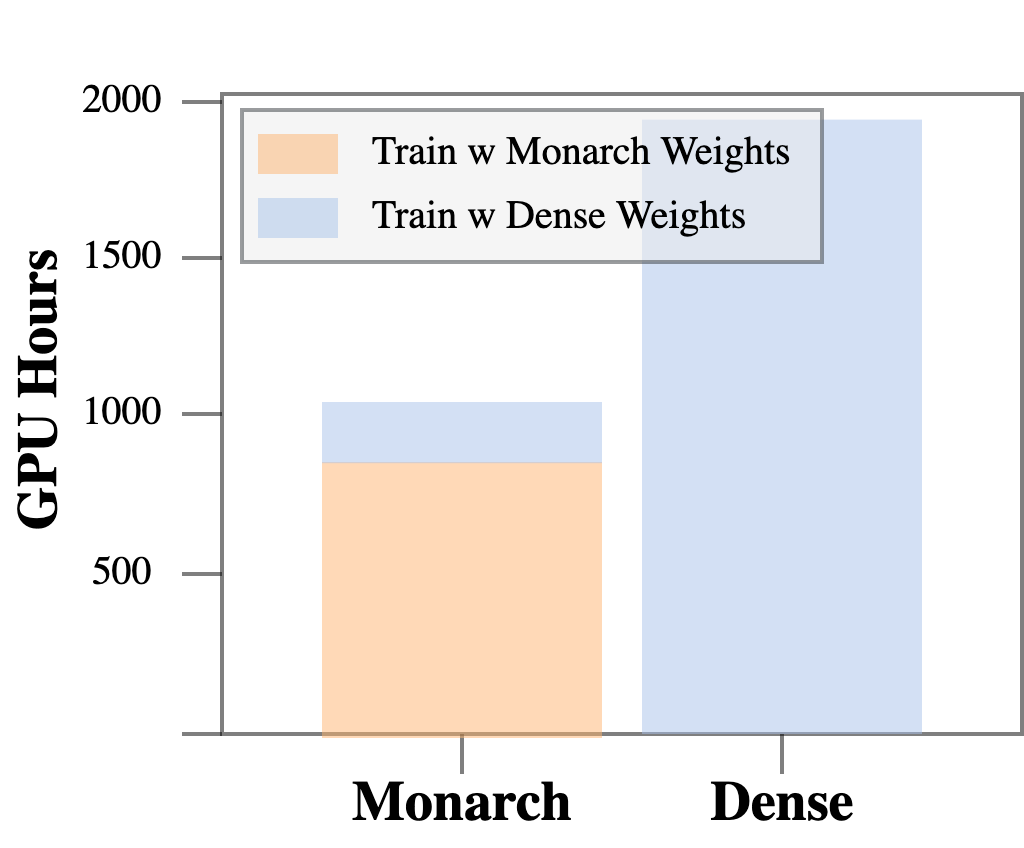
\includegraphics[width=.3\textwidth]{figures/rv_bar_temp.png}
  \vspace{-3mm}
  \caption{\label{fig:reverse_sparsification_bar}Time required (in A100 GPU hours) to reach the same perplexity (18.0)
    for GPT-2-small on OpenWebText.
    With ``reverse sparsification'', Monarch can speed up
    GPT-2 training by 2$\times$.\vspace{-1em}}
\end{figure}

We show that our Monarch approximation algorithm allows us to efficiently use
pretrained models, such as speeding up BERT finetuning on GLUE.

\paragraph{BERT finetuning.}
We take the BERT pretrained weights, approximate them with Monarch matrices,
and finetune the resulting model on the 9 GLUE tasks.
The results in \cref{table:bert_glue} shows that we obtain a Monarch finetuned
model with similar quality to the dense BERT model, but with 1.7$\times$ faster
finetuning speed.
This serves as a proof of concept, and we expect further speedup if additional model compression techniques are applied (e.g., quantization, kernel fusion).




\begin{table}[h]
  \small
  \centering
  \vspace{-5mm}
  \caption{\label{table:bert_glue}The performance of Monarch matrices in
    finetuning BERT on GLUE.}
  \setlength{\tabcolsep}{5pt}
  \vspace{1em}
  \iftoggle{arxiv}{}{
    \resizebox{\linewidth}{!}
  }
  {
  \begin{tabular}{@{}c||ccccccc@{}}
  \specialrule{.15em}{.05em}{.05em}
    Model&\multicolumn{1}{c}{GLUE (avg)}&\multicolumn{1}{c}{Speedup} &\multicolumn{1}{c}{Params} & \multicolumn{1}{c}{FLOPs} \\
    \specialrule{.15em}{.05em}{.05em}
    BERT-base & 78.6& - & 109M & 11.2G \\
    Monarch-BERT-base& 78.3& 1.5$\times$ & 55M & 6.2G  \\
    BERT-large & 80.4 & - & 335M & 39.5G \\
    Monarch-BERT-large & 79.6 & 1.7$\times$ & 144M & 14.6G  \\
    \specialrule{.15em}{.05em}{.05em}
  \end{tabular}
  }
  \vspace{-3mm}
\end{table}




\section{Conclusion and Future Work}
\label{sec:conclusion}

Hyperbolic embeddings embed hierarchical information with high
fidelity and few dimensions. We explored the limits of this approach
by describing scalable, high quality algorithms. We hope the
techniques here encourage more follow-on work on the exciting
techniques of \citet{fb, ucl}. As future work, we hope to explore how
hyperbolic embeddings can be most effectively incorporated into downstream
tasks and applications.


\bibliographystyle{plainnat}
\bibliography{hyperbolic_bib}

\pagebreak

\appendix
\appendix

% \section{Claimed Emergent Abilities}
% \label{app:claimed_emergent_abilities}

% We compile the models, tasks and metrics that different papers have claimed reveal emergent abilities of large language models. This list may be incomplete or inaccurate, but represents a good faith attempt to compile this information. Note: quantifying model scale when an ability emerges is complicated by the fact that different papers report model scale differently, either as (a) number of parameters \cite{brown2020language, ganguli2022predictability}, (b) effective number of parameters \cite{srivastava2022beyond} or (c) training FLOPs \cite{wei2022emergent}.

% \begin{table}[h!]
%     \centering
%     \begin{tabular}{|l|c|c|c|}
%     \hline
%         Task & Model Families & Metric & Model Scale at Emergence \\
%         \hline
%         2-Digit Addition \cite{brown2020language} & GPT-3 & Accuracy & 13B Parameters\\
%         2-Digit Subtraction \cite{brown2020language} & GPT-3 & Accuracy & 13B Parameters\\
%         3-Digit Addition \cite{brown2020language, ganguli2022predictability} & GPT-3 & Accuracy & 175B Parameters\\
%         3-Digit Subtraction \cite{brown2020language} & GPT-3 & Accuracy & 175B Parameters\\
%         MMLU \cite{ganguli2022predictability} & GPT-3, Gopher & Accuracy & 200B, 300B Parameters\\
%         Program Synthesis \cite{ganguli2022predictability} & Google Internal & \% Samples Solving Task & 200B Parameters\\
%         Figure of Speech Detection \cite{srivastava2022beyond} & ? & ? & $\sim 10^{11}$ Effective Parameters \\
%         IPA Transliterate \cite{srivastava2022beyond, wei2022emergent} & LaMDA, GPT-3 & BLEU & $\sim 10^{23}, \sim 10^{23}$ Training FLOPs\\
%         Periodic Elements \cite{srivastava2022beyond} & ? & ? & ?\\
%         Modified Arithmetic \cite{srivastava2022beyond, wei2022emergent} & GPT-3, LaMDA & Accuracy & $\sim 10^{23}, \sim 10^{24}$ Training FLOPs\\
%         Repeat Copy Logic \cite{srivastava2022beyond} & ? & ? & $10^{11}$ Effective Parameters\\
%         Word Unscrambling \cite{srivastava2022beyond, wei2022emergent} & LaMDA & Exact Match & $\sim 10^{24}$ Training FLOPs\\
%         Persian QA \cite{wei2022emergent} & PaLM & Exact Match & $\sim 10^{24}$ Training FLOPs\\
%         Truthful QA \cite{wei2022emergent} & Gopher & Accuracy & $\sim 10^{23}$ Training FLOPs\\
%         Grounded Mappings \cite{wei2022emergent} & ? & ? & ?\\
%         Multi-task NLU \cite{wei2022emergent} & ? & ? & ?\\
%         Word in context \cite{wei2022emergent} & ? & ? & $\sim 10^{24}$ Training FLOPs\\
%         \hline
%     \end{tabular}
%     \newline
%     \caption{\textbf{Tasks, model families, metrics and number of parameters for emergent abilities.}}
%     \label{tab:my_label}
% \end{table}


% \section{Exponentiated Negative Cross Entropy Lower Bounds Accuracy}
% \label{app:acc_bound}

% Consider batch size $B$ with length $L$. During training i.e. with teacher-forcing, the per-token accuracy (averaged over batch index $b$ and sequence index $l$) is defined as:
% %
% \begin{align}
%     \text{Acc} &\defeq \frac{1}{B} \sum_b \frac{1}{L} \sum_l p(t_{bl}^* | t_{b, <l}^*)\\
%     &= \frac{1}{BL} \sum_{b, l} p(t_{bl}^* | t_{b, <l}^*)
% \end{align}

% The cross entropy (commonly averaged over the batch) is defined as:
% %
% \begin{align}
%     \mathcal{L}_{CE} &\defeq -\frac{1}{B} \sum_b \log p(t_{b 1}^*, ..., t_{b L}^*)\\
%     &= -\frac{1}{B} \sum_b \log \prod_l p(t_{b l}^*| t_{b, <l}^*)\\
%     &= -\frac{1}{B} \sum_{b, l} \log p(t_{bl}^* | t_{b, <l}^*)
% \end{align}

% To make the comparison between accuracy and cross entropy a little easier, let's normalize the cross entropy by the sequence length:
% %
% \begin{align}
%     \mathcal{L}_{CE/L} &\defeq \frac{1}{L}\mathcal{L}_{CE}\\
%     &=  -\frac{1}{BL} \sum_{b, l} \log p(t_{bl}^* | t_{b, <l}^*)
% \end{align}

% Recall that Jensen's inequality tells us that for any random variable $X$, $\log \mathbb{E}[X] \geq \mathbb{E}[\log X]$. The relationship between sequence-length-normalized cross entropy and accuracy is thus:
% %
% \begin{align}
%     -\mathcal{L}_{CE/L} = \frac{1}{BL} \sum_{b, l} \log p(t_{bl}^* | t_{b <l}^*) &\leq \log \frac{1}{BL} \sum_{b, l}  p(t_{bl}^* | t_{b <l}^*) = \log \text{Acc}\\
%     \exp(- \mathcal{L}_{CE/L}) &\leq \text{Acc}
% \end{align}

% Consequently, we see that driving the cross entropy loss to $0$ necessarily drives the accuracy to $1$.

% TODO: Can we use the second moment method to derive bounds on how (un)likely a subset of tokens are to deviate from the mean?


\section{Approximate Behavior of Metrics on Sequential Data}
\label{app:metric_scaling}

How do different metrics behave when used to measure autoregressive model outputs? Precisely answering this question is tricky and possibly analytically unsolvable, so we provide an approximate answer here.

Notationally, we consider $N$ test data of length $L$ (here, length is measured in tokens) with targets denoted $t_n \defeq (t_{n1}, t_{n2}, ... t_{nL})$, the autoregressive model has a true-but-unknown per-token error probability of $\epsilon \in [0, 1]$ and the model outputs prediction $\hat{t}_n \defeq (\hat{t}_{n1}, \hat{t}_{n2}, ... \hat{t}_{nL})$. This assumes that the model's per-token error probability is constant, which is empirically false, but modeling the complex dependencies of errors is beyond our scope.

\subsection{Per-Token Error Probability is Resolution-Limited}
\label{app:metric_scaling:resolution_limited}

Note that because we have $N$ test data, each of length $L$, our resolution for viewing the per-token error probability $\epsilon$ is limited by $1/NL$. 
Here, resolution refers to ``the smallest interval measurable by a scientific instrument; the resolving power."
To explain what resolution means via an example, suppose one wants to measure a coin's probability of yielding heads.
After a single coin flip, only two outcomes are possible (H, T), so the resolution-limited probability of heads is either $0$ or $1$.
After two coin flips, four outcomes are possible (HH, HT, TH, TT), so the resolution-limited probability of heads is now one of $0, 0.5, 1$.
After $F$ coin flips, we can only resolve the coin's probability of yielding heads up to $1/F$.
Consequently, we introduce a resolution-limited notation:
%
\begin{equation}
    \nint{a}_b \defeq \text{$a$ rounded to the nearest integer multiple of $1/b$}
\end{equation}

\subsection{Token Edit Distance}
\label{app:metric_scaling:token_edit_distance}

We first consider an adaptation of the Levenshtein (string edit) distance for models that function on tokens rather than characters, an adaptation we term the \textit{token edit distance}. The token edit distance between two token sequences $t_n, \hat{t_n}$ is defined as the integer number of additions, deletions or substitutions necessary to transform $t_n$ into $\hat{t}_n$ (or vice versa).

\begin{align}
    \text{Token Edit Distance}(t_n, \hat{t}_n)  &\defeq \text{Num Substitutions} + \text{Num. Additions} + \text{Num. Deletions}\\
    &= \sum_{\ell =1}^L \mathbb{I}[t_{n\ell} \neq \hat{t}_{n\ell}] + \text{Num. Additions} + \text{Num. Deletions}\\
    &\geq \sum_{\ell =1}^L \mathbb{I}[t_{n\ell} \neq \hat{t}_{n\ell}]
\end{align}

The expected token edit distance is therefore:

\begin{align}
    \mathbb{E}[\text{Token Edit Distance}(t_n, \hat{t}_n)] &\geq \mathbb{E}[\sum_{\ell =1}^L \mathbb{I}[t_{n\ell} \neq \hat{t}_{n\ell}]]\\
    &= \sum_{\ell =1}^L p(t_{n\ell} \neq \hat{t}_{n\ell})\\
    &\approx L (1 - \epsilon)
\end{align}

The resolution-limited expected token edit distance is therefore:

\begin{equation}
    \nint{\mathbb{E}[\text{Token Edit Distance}(t_n, \hat{t}_n)]}_{NL} \geq L \Big(1 - \nint{\epsilon}_{NL} \Big)
\end{equation}

From this, we see that the expected token edit distance scales approximately linearly with the resolution-limited per-token probability. The real rate is slightly higher than linear because additions and deletions contribute an additional non-negative cost, but modeling this requires a model of how likely the model is to overproduce or underproduce tokens, which is something we do not currently possess.

\subsection{Accuracy}
\label{app:metric_scaling:accuracy}

\begin{align}
    \text{Accuracy}(t_n, \hat{t}_n) &\defeq \mathbb{I}[\text{No additions}] \, \mathbb{I}[\text{No deletions}] \, \prod_{l=1}^L \mathbb{I}[t_{nl} = \hat{t}_{nl}]\\
    &\approx \prod_{l=1}^L \mathbb{I}[t_{nl} = \hat{t}_{nl}]
\end{align}

As with the Token Edit Distance (App. \ref{app:metric_scaling:accuracy}), we ignore how likely the language model is to overproduce or underproduce tokens because we do not have a good model of this process. Continuing along,

\begin{align}
    \mathbb{E}[\log \text{Accuracy}] &= \sum_l \mathbb{E}[\log \mathbb{I}[t_{nl} = \hat{t}_{nl}]]\\
    &\leq \sum_l \log \mathbb{E}[\mathbb{I}[t_{nl} = \hat{t}_{nl}]]\\
    &\approx L \log (1- \epsilon)
    % \exp(\mathbb{E}[\log \text{Accuracy}]) &= \exp (\sum_l \mathbb{E}[\log \mathbb{I}(t_{nl}, \hat{t}_{nl})])\\
    % &=
\end{align}

Taking an approximation that would make most mathematicians cry:

\begin{align}
    \mathbb{E}[\text{Accuracy}] &\approx \exp(\mathbb{E}[\log \text{Accuracy}])\\
    &= (1 - \epsilon)^L\\
\end{align}

This reveals that accuracy \textbf{approximately} falls geometrically with target token length. The resolution-limited expected accuracy is therefore:

\begin{equation}
    \nint{\mathbb{E}[\text{Accuracy}]}_{NL} = \nint{(1 - \epsilon)^L}_{NL}
\end{equation}

From this we can see that choosing a nonlinear metric like Accuracy is affected significantly more by limited resolution because Accuracy forces one to distinguish quantities that decay rapidly.

\subsection{ROUGE-L-Sum}
\label{app:metric_scaling:rougeLsum}

\begin{figure}
    \centering
    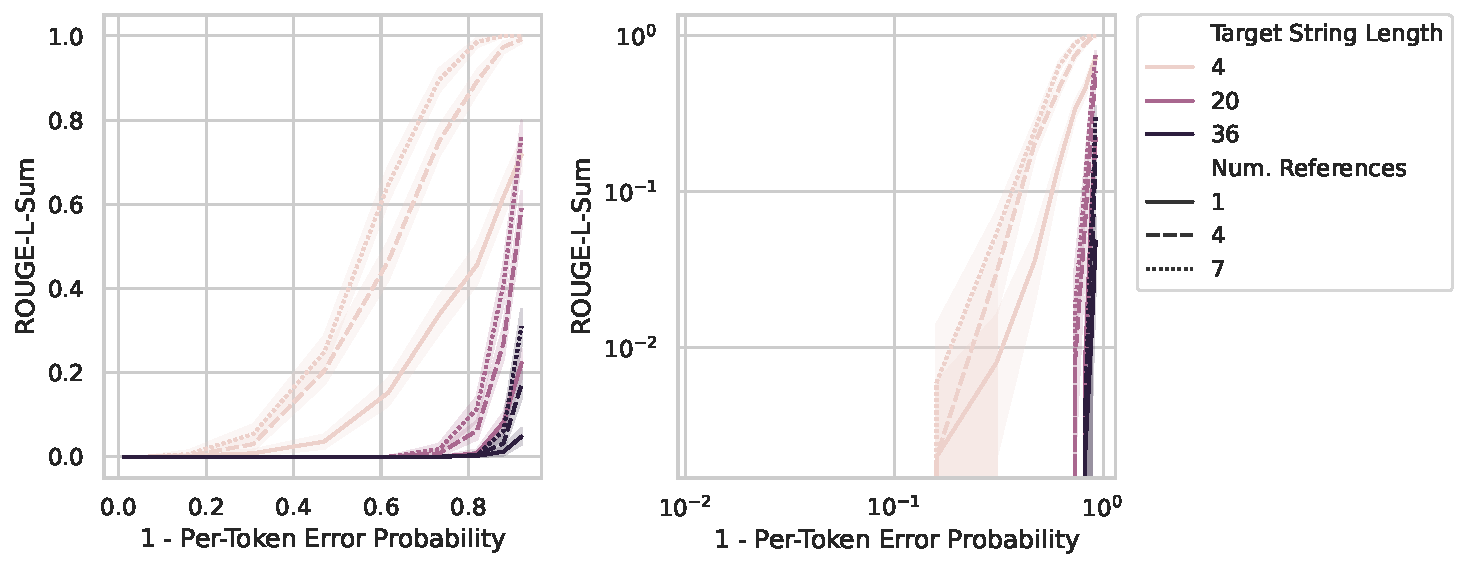
\includegraphics[width=0.95\textwidth]{figures/rouge_understanding/rougeLsum_vs_token_error_prob_scaling_simulation.pdf}
    \caption{\textbf{ROUGE-L-Sum is a sharp metric.} Simulations show that as the per-token error probability slightly increase (e.g. from 0.05 to 0.1), the ROUGE-L-Sum metric sharply falls.}
    \label{fig:app:metric_scaling:rougeLsum}
\end{figure}


Another BIG-Bench metric \cite{srivastava2022beyond} is ROUGE-L-Sum \cite{lin2004rouge}, a metric based on the longest common subsequence (LCS) between two sequences. Section 3.2 of \cite{lin2004rouge} gives the exact definition, but the key property is that ROUGE-L-Sum measures the ``union" LCS, which means ``stitching" together LCSs across the candidate and multiple references. As explained in the original paper: if the candidate sequence is $c = w_1 w_2 w_3 w_4 w_5$, and if there are two reference sequences $r_1 = w_1 w_2 w_6 w_7 w_8$ and $r_2 = w_1 w_3 w_8 w_9 w_5$, then $LCS(r_1, c) = w_1 w_2$ and $LCS(r_2, c) =w_1 w_3 w_5$, then the \textit{union} 
-LCS of $c, r_1, r_2$ is $w_1 w_2 w_3 w_5$, with length 4. Intuitively, this disproportionately benefits models with smaller error rates because their mistakes can be ``stitched" across multiple references; this is confirmed in simulation (Fig. \ref{fig:app:metric_scaling:rougeLsum}).


% \subsection{BLEU}
% \label{app:metric_scaling:bleu}


% \subsection{Emergence does not require on scaling laws: decreasing cross-entropy loss and stricter exact match is all you need }

% The goal of this section is to show that scaling laws are not necessary to create emergence and that many functional forms of the loss are valid as long as the form decreases as some other variable decreases -- say the number of parameters in the model.
% This typically holds in modern machine learning. 
% We do this by considering different functional forms of the cross entropy $CE(N)$, as a function of the number of parameters $N$, and show emergence, i.e. sharpness and unpredictability.
% We illustrate this by showing the programmer can exaggerate the sharpness (and therefore emergence) by implying increasing the exact number of tokens required to get correct in the accuracy, i.e. increasing $L$ in our notation.

% \subsubsection{Argument}

% Recall from section \ref{sec:alt_explanation} the accuracy requiring all $L$ tokens to be correct for a model of size $N$ as a function of cross-entropy $CE(N)$:

% \begin{equation*}
%     \text{Accuracy}(N) \approx p_N(\text{single token correct})^{\text{num. of tokens}} = \exp \Big(- CE(N) \Big)^L
% \end{equation*}

% We plot this equation using three functional forms for a decreasing cross-entropy loss in figure \ref{fig:decreasing_loss_leads_to_emergence_as_L_increases} for increasing values of $L$.
% These increasing values of $L$ induce a sharper -- therefore, seemingly more emergent curve when plotting the accuracy. 
% This means that if the programmer simply requires a stricter accuracy, he can make a perfectly smooth and predictable cross-entropy loss suddenly become sharp and unpredictable, i.e. ``emergent". 
% We show numerically it is independent of the functional form and instead that it only requires the cross-entropy to be decreasing and the accuracy metric to have some non-linear transformation that makes it sharper. 
% Therefore, if one had only tracked the cross-entropy loss instead, one could have had a smooth predictable curve for the models.
% This implies small-scale experimentation is still relevant, and we wish to highly that GPT-4 \cite{gpt4} small-scale experiment in conjunction with scaling loss. 
% We'd like to emphasize that changing the evaluation metric can suddenly induce emergence, and it is not an intrinsic property of the model. 

% %The goal will be to show that if $CE(N)$ decreases with different functional forms that $acc$ is emergent (either sharp or unpredictable).
% % TODO: sharp due to L
% % TODO: unpredictable due to constant and L

% \begin{figure}[htbp]
%   \centering
%   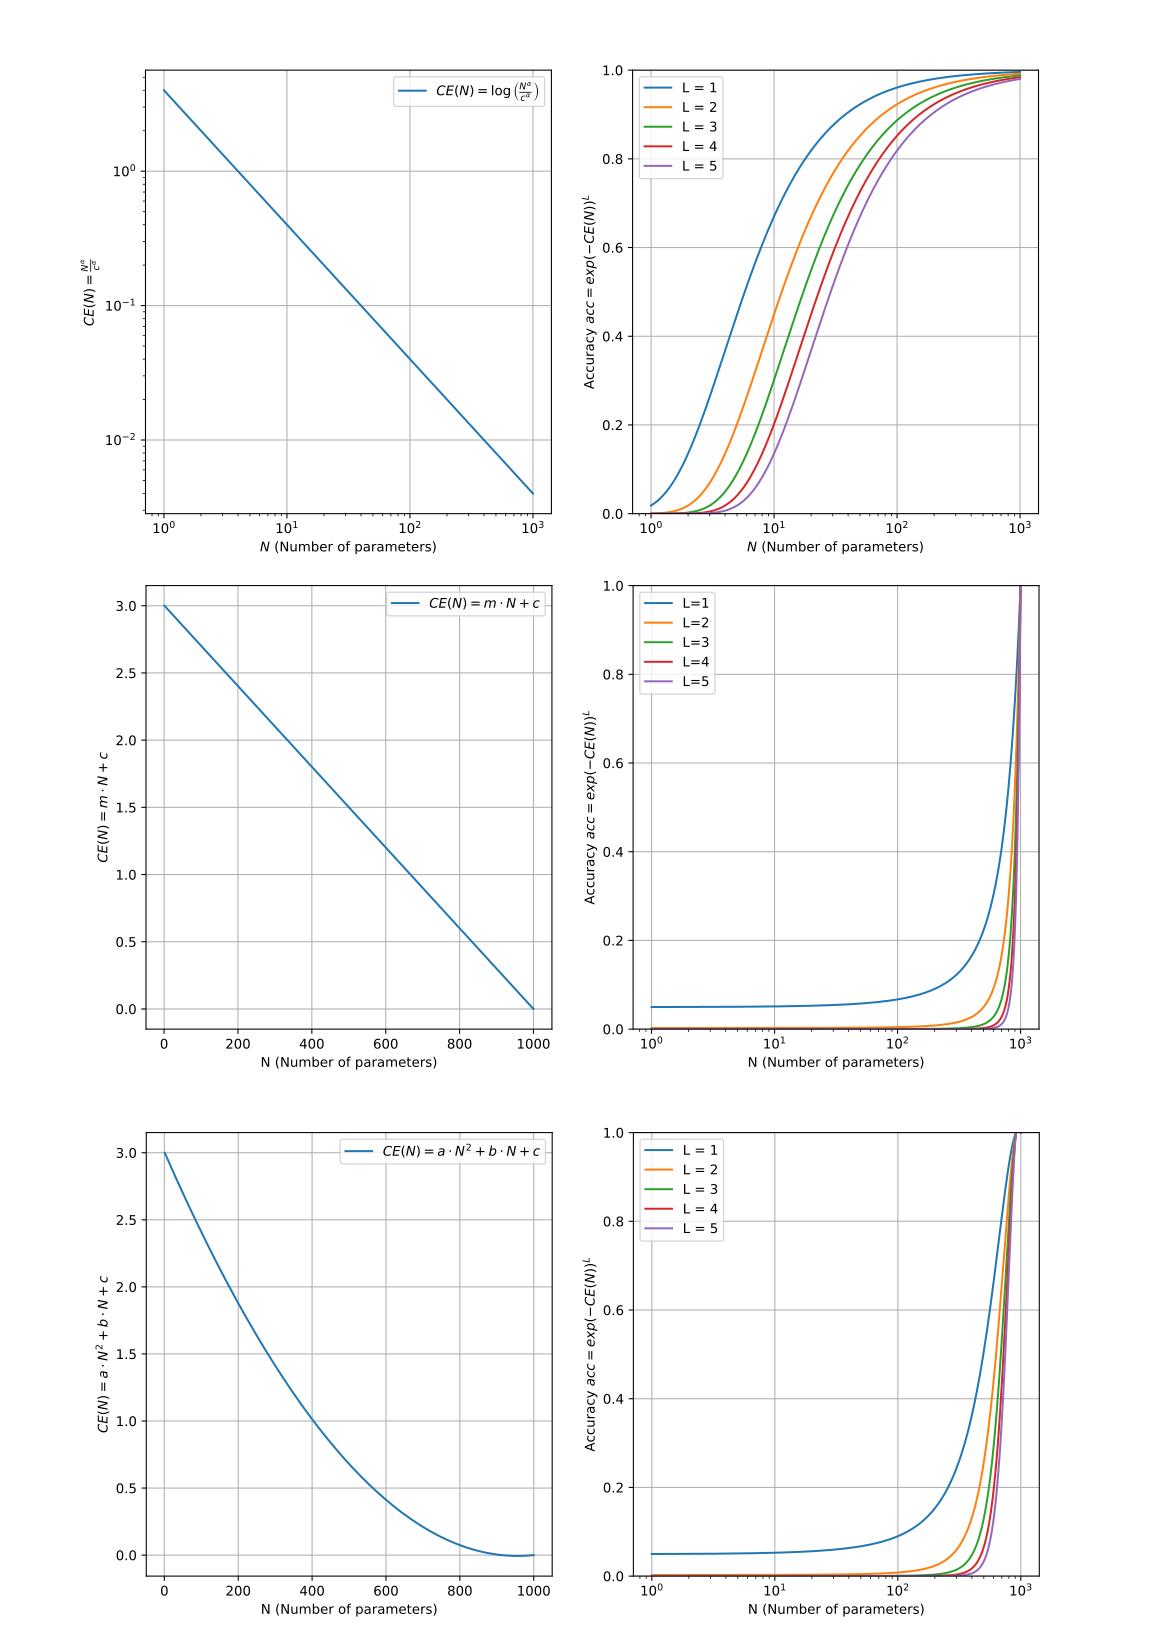
\includegraphics[width=0.8\textwidth]{figures/loss_decreasing_leads_to_emergence/decreasing_loss_leads_to_emergence_as_L_increases.png}
%   \caption{
%   \textbf{Emergence does not depend on scaling laws: any decreasing cross-entropy loss induces apparent emergence as L increases as you require more tokens to be exactly correct, i.e. L increases.}
%   The first row shows the same argument as in the main section, where a decreasing cross-entropy loss as a scaling law induces emergence as $L$ increases.
%   The second row shows the that apparent emergence is induced even when the cross-entropy loss decreases linearly.
%   The third row shows that the apparent emergence is induced when the cross-entropy loss decreases quadratically.
%   Emergence is amplified in this case especially by the increase in sharpness as more tokens are required to be correct. 
%   This means that simply changing the evaluation metric can suddenly induce emergence, and it is not an intrinsic property of the model. 
%   }
%   \label{fig:decreasing_loss_leads_to_emergence_as_L_increases}
% \end{figure}


\section{Inducing Emergent Abilities in Networks on Vision Tasks}
\label{app:sec:inducing_emergence_vision}

\subsection{Emergent Classification of MNIST Handwritten Digits by Convolutional Networks}

\begin{figure}
    \centering
    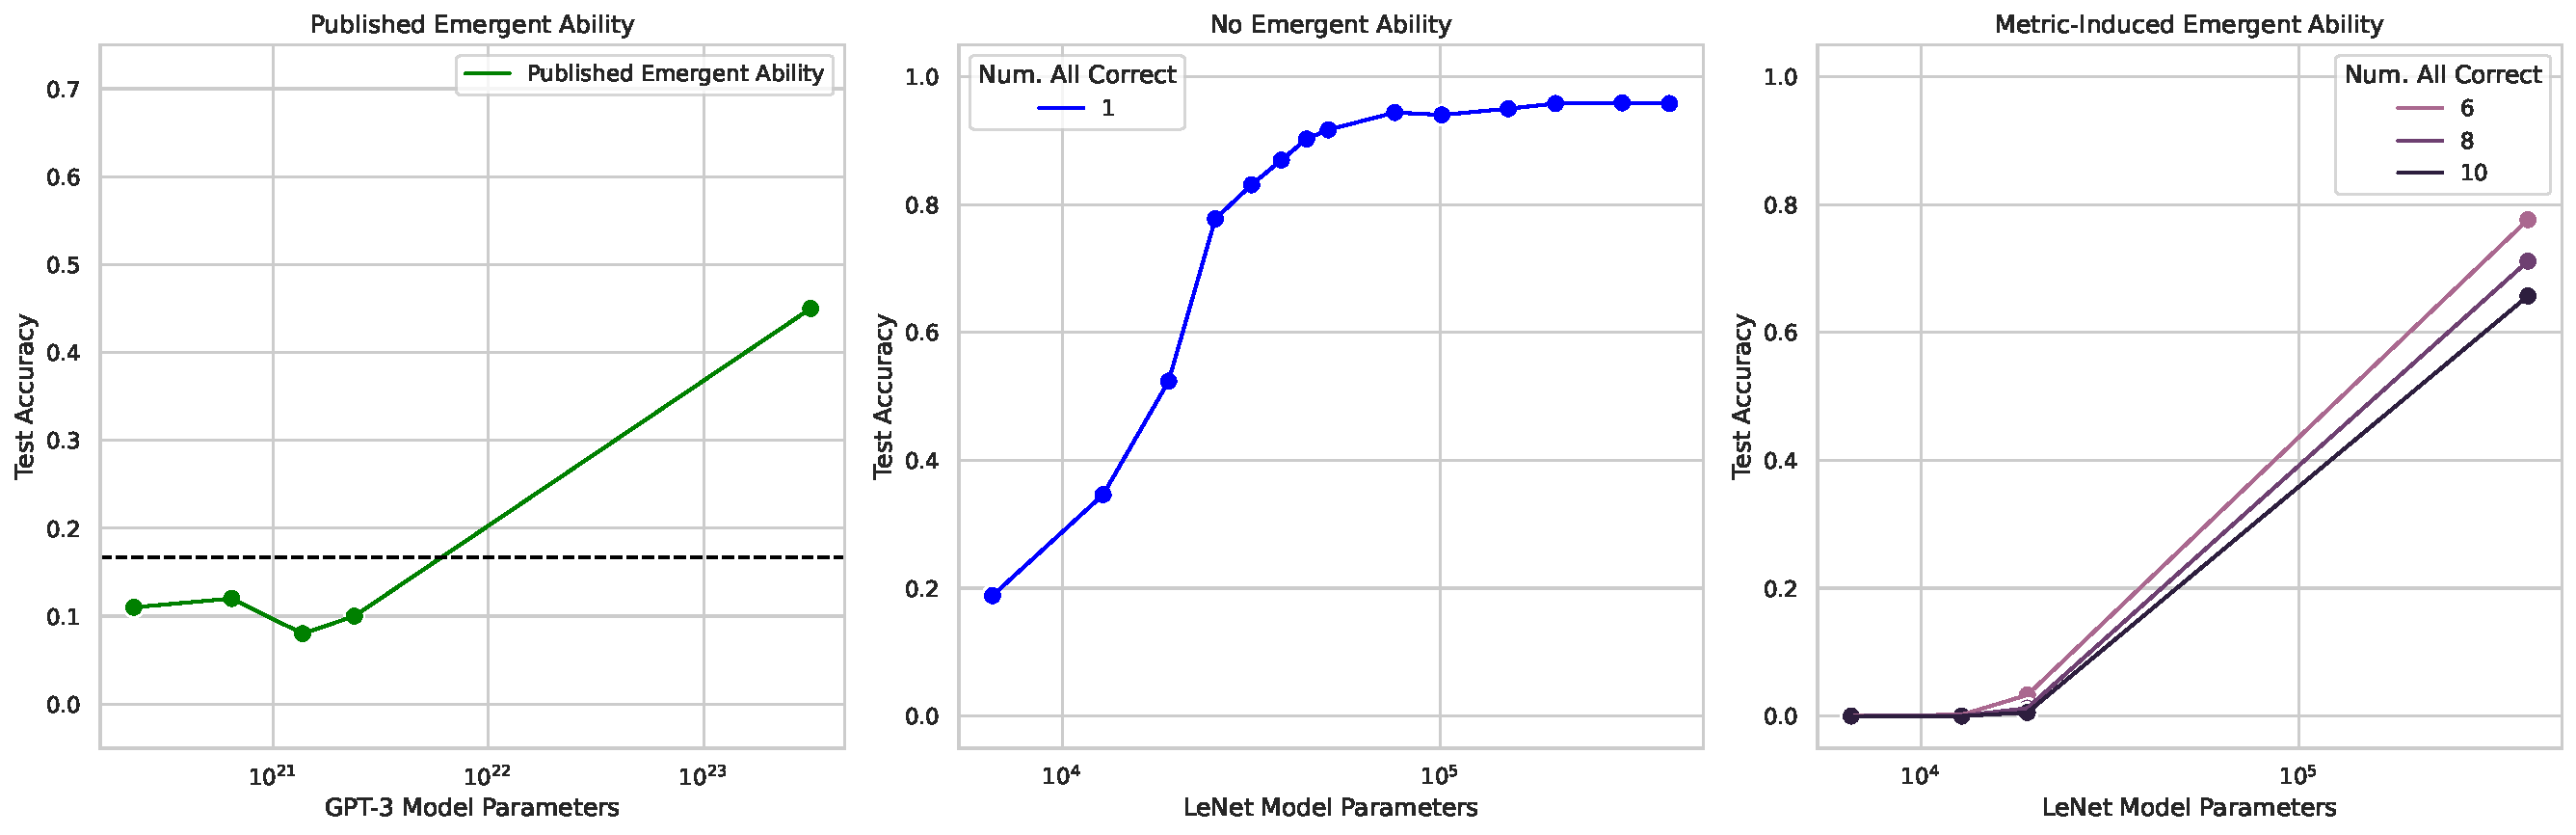
\includegraphics[width=\textwidth]{figures/vision/no_emergence_and_emergence_dataset=mnist.pdf}
    \caption{\textbf{Induced emergent MNIST classification ability in convolutional networks.} (A) A published emergent ability from the BIG-Bench Grounded Mappings task \cite{wei2022emergent}. (B) LeNet trained on MNIST \cite{lecun1998mnist} displays a predictable, commonplace sigmoidal increase in test accuracy as model parameters increase. (C) When accuracy is redefined as correctly classifying $K$ out of $K$ independent test data, this newly defined metric induces a seemingly unpredictable change.}
    \label{fig:vision_mnist}
\end{figure}

We begin by inducing an emergent classification ability in a LeNet convolutional neural network family \cite{lecun1998gradient}, trained on the MNIST handwritten digits dataset \cite{lecun1998mnist}.
This family displays smoothly increasing test accuracy as the number of parameters increase (Fig. \ref{fig:vision_mnist}B).
To emulate the accuracy metric used by emergence papers \cite{ganguli2022predictability, wei2022emergent, srivastava2022beyond}, we use \textit{subset accuracy}: 1 if the network classifies $K$ out of $K$ (independent) test data correctly, 0 otherwise.
Under this definition of accuracy, the model family displays an ``emergent" ability to correctly classify sets of MNIST digits as $K$ increases from $1$ to $5$, especially when combined with sparse sampling of model sizes (Fig. \ref{fig:vision_mnist}C).
This convolutional family's emergent classification ability qualitatively matches published emergent abilities, e.g., at the BIG-Bench Grounded Mappings task \cite{wei2022emergent} (Fig. \ref{fig:vision_mnist}A).


\end{document}
